%%%%%%%%%%%%%%%%%%% vorlage.tex %%%%%%%%%%%%%%%%%%%%%%%%%%%%%
%
% LaTeX-Vorlage zur Erstellung von Projekt-Dokumentationen
% im Fachbereich Informatik der Hochschule Trier
%
% Basis: Vorlage svmono des Springer Verlags
%
%%%%%%%%%%%%%%%%%%%%%%%%%%%%%%%%%%%%%%%%%%%%%%%%%%%%%%%%%%%%%

\documentclass[envcountsame,envcountchap, deutsch]{i-studis}

\usepackage{makeidx}         	% Index
\usepackage{multicol}        	% Zweispaltiger Index
%\usepackage[bottom]{footmisc}	% Erzeugung von Fu�noten

%%-----------------------------------------------------
%\newif\ifpdf
%\ifx\pdfoutput\undefined
%\pdffalse
%\else
%\pdfoutput=1
%\pdftrue
%\fi
%%--------------------------------------------------------
%\ifpdf
\usepackage[pdftex]{graphicx}
\usepackage[pdftex,plainpages=false]{hyperref}
%\else
%\usepackage{graphicx}
%\usepackage[plainpages=false]{hyperref}
%\fi

%%-----------------------------------------------------
\usepackage{color}				% Farbverwaltung
%\usepackage{ngerman} 			% Neue deutsche Rechtsschreibung
\usepackage[english, ngerman]{babel}
\usepackage[latin1]{inputenc} 	% Erm�glicht Umlaute-Darstellung
%\usepackage[utf8]{inputenc}  	% Erm�glicht Umlaute-Darstellung unter Linux (je nach verwendetem Format)

%-----------------------------------------------------
\usepackage{listings} 			% Code-Darstellung
\lstset
{
	basicstyle=\scriptsize, 	% print whole listing small
	keywordstyle=\color{blue}\bfseries,
								% underlined bold black keywords
	identifierstyle=, 			% nothing happens
	commentstyle=\color{red}, 	% white comments
	stringstyle=\ttfamily, 		% typewriter type for strings
	showstringspaces=false, 	% no special string spaces
	framexleftmargin=7mm, 
	tabsize=3,
	showtabs=false,
	frame=single, 
	rulesepcolor=\color{blue},
	numbers=left,
	linewidth=146mm,
	xleftmargin=8mm,
	breaklines=true,
	language=Lisp
}
\usepackage{textcomp} 			% Celsius-Darstellung
\usepackage{amssymb,amsfonts,amstext,amsmath}	% Mathematische Symbole
\usepackage[german, ruled, vlined]{algorithm2e}
\usepackage[a4paper]{geometry} % Andere Formatierung
\usepackage{bibgerm}
\usepackage{array}
\hyphenation{Ele-men-tar-ob-jek-te  ab-ge-tas-tet Aus-wer-tung House-holder-Matrix Le-ast-Squa-res-Al-go-ri-th-men} 		% Weitere Silbentrennung bei Bedarf angeben
\setlength{\textheight}{1.1\textheight}
\pagestyle{myheadings} 			% Erzeugt selbstdefinierte Kopfzeile
\makeindex 						% Index-Erstellung


%--------------------------------------------------------------------------
\begin{document}
%------------------------- Titelblatt -------------------------------------
\title{Konzeption und Implementierung eines Systems zur automatischen Analyse und Klassifikation von Berichten in Nachrichtenportalen}
\subtitle{Conception and implementation of a system for the automatic analysis and classification of articles in newsportals}
%---- Die Art der Dokumentation kann hier ausgew�hlt werden---------------
%\project{Bachelor-Projektarbeit}
\project{Bachelor-Abschlussarbeit}
%\project{Master-Projektstudium}
%\project{Master-Abschlussarbeit}
%\project{Seminar zur Vorlesung ...}
%\project{Hausarbeit zur Vorlesung ...}
%--------------------------------------------------------------------------
\supervisor{Karl Hans Blaesius} 		% Betreuer der Arbeit
\author{Tobias Arens} 							% Autor der Arbeit
\address{Trier,} 							% Im Zusammenhang mit dem Datum wird hinter dem Ort ein Komma angegeben
\submitdate{13.12.2016} 				% Abgabedatum
%\begingroup
%  \renewcommand{\thepage}{title}
%  \mytitlepage
%  \newpage
%\endgroup
\begingroup
  \renewcommand{\thepage}{Titel}
  \mytitlepage
  \newpage
\endgroup
%--------------------------------------------------------------------------
\frontmatter 
%--------------------------------------------------------------------------
%\preface

Ein Vorwort ist nicht unbedingt n�tig. Falls Sie ein Vorwort schreiben, so ist dies der Platz, um z.B. die Firma vorzustellen, in der diese Arbeit entstanden ist, oder einigen Leuten zu danken, die in irgendeiner Form positiv zur Entstehung dieser Arbeit beigetragen haben. Auf keinen Fall sollten Sie im Vorwort die Aufgabenstellung n�her erl�utern oder vertieft auf technische Sachverhalte eingehen.				% Vorwort (optional)
\kurzfassung

%% deutsch
\paragraph*{}

In dieser Arbeit wurde eine erweiterte Variante des Klassifikationsalgorithmus Naive-Bayes implementiert. Aus in Textdateien vorliegenden Konfigurationsdaten wird dynamsich ein Klassifikationskorpus erzeugt, der es erm�glicht aktuelle Nachrichtenartikel verschiedener Onlineportale zu klassifizieren.
Mithilfe einer simplen graphischen Benutzeroberfl�che ist es m�glich diese Artikel zu durchsuchen und einen Einblick in die zugrunde liegenden Daten zu gewinnen. 
Ben�tigte Grundlagen der Textklassifikation sowie das Vorgehen bei Konzeption und Realisierung der Arbeit werden ausf�hrlich beschrieben.

%% englisch
\paragraph*{}
This paper shows an implementation of an advanced variant of the Naive-Bayes classification algorithm. Through available configuration files a classification corpus is dynamically generated by which it is possible to classify current news from online news portals. 
A simple graphical-user-interface allows it to filter the results of this search and makes the underlying data easily accessible.
Required fundamentals of text-classification and the approach of design and implementation of this work are described in detail. 			% Kurzfassung Deutsch/English
\tableofcontents 						% Inhaltsverzeichnis
\listoffigures 							% Abbildungsverzeichnis (optional)
\listoftables 							% Tabellenverzeichnis (optional)
%--------------------------------------------------------------------------
\mainmatter                        		% Hauptteil (ab hier arab. Seitenzahlen)
%--------------------------------------------------------------------------
% Die Kapitel werden in separaten .tex-Dateien abgelegt und hier eingebunden.
\chapter{Einleitung und Problemstellung}

%Begonnen werden soll mit einer Einleitung zum Thema, also Hintergrund und Ziel erl�utert werden.

%Weiterhin wird das vorliegende Problem diskutiert: Was ist zu l�sen, warum ist es wichtig, dass man dieses Problem l�st und welche L�sungsans�tze gibt es bereits. Der Bezug auf vorhandene oder eben bisher fehlende L�sungen begr�ndet auch die Intention und Bedeutung dieser Arbeit. Dies k�nnen allgemeine Gesichtspunkte sein: Man liefert einen Beitrag f�r ein generelles Problem oder man hat eine spezielle Systemumgebung oder ein spezielles Produkt (z.B. in einem Unternehmen), woraus sich dieses noch zu l�sende Problem ergibt.

%Im weiteren Verlauf wird die Problemstellung konkret dargestellt: Was ist spezifisch zu l�sen? Welche Randbedingungen sind gegeben und was ist die Zielsetzung? Letztere soll das
%beschreiben, was man mit dieser Arbeit (mindestens) erreichen m�chte.


%Zur Informationsbeschaffung in der heutigen Zeit gibt es zahlreiche M�glichkeiten. So gibt es hunderte Online-Nachrichtenportale, Zeitschriften, Zeitungen und Magazine aus denen wertvolle Informationen gewonnen werden k�nnen. 

%Diese Diversit�t hat viele positive Eigenschaften, wie das vorliegen verschiedener Standpunkte und die Beleuchtung von Ereignissen und Nachrichten aus vielen Blickrichtungen. Die dadurch erreichte Abdeckung ist begr��enswert, schafft allerdings einige Probleme. 
In der heutigen Zeit gibt es viele M�glichkeiten an Informationen �ber Themen aller Art zu gelangen. So besteht neben einer gro�en Vielfalt an Zeitungen, Zeitschriften und Magazinen auch die M�glichkeit, sich �ber Online-Quellen, wie Informationsportale oder Webpr�senzen von Zeitungen zu informieren.

Diese Diversit�t hat die Folge, dass eine sehr gro�e Bandbreite an Themen aus verschiednen Blickwinkeln beleuchtet und somit eine relativ unabh�ngige Informationsbeschaffung erm�glicht wird. \\
Doch diese Vielfalt an Informationsquellen bringt auch die Schwierigkeit mit sich, sich gezielt �ber ein bestimmtes Thema zu informaieren, ohne die Diversit�t verschiedener Meinungen und Blickpunkte aufgeben zu m�ssen.
Es ist umst�ndlich bei Interesse an einem bestimmten Thema passende Artikel zu finden da daf�r eine M�glichkeit einer gro�fl�chigen Abdeckung verschiedener Portale fehlt.\\


Um Artikel thematisch zuordnen zu k�nnen, ist eine automatisierte Klassifizierung sinnvoll, die diese Artikel zielsicher mithilfe vorab definierter Klassen abbilden kann. Dies erm�glicht eine zielgerichtete, breitgef�cherte Suche nach themenbezogenen Informationen.\\


In Rahmen dieser Arbeit wird mithilfe der funktionalen Programmiersprache Lisp eine Anwendung entwickelt, die dieses Problem l�sen soll. 
Daf�r sind allerdings mehrere Schritte notwendig: 
es muss eine Schnittstelle entwickelt werden, die Nachrichtenartikel verschiedener Quellen auslesen kann, um diese f�r die weitere Verarbeitung nutzen zu k�nnen.
Die so gewonnenen Daten m�ssen mit entsprechenden Metriken bewertet und mithilfe eines Klassifizierungsalgorithmus korrekt zugeordnet werden.
Um dies zu erm�glichen, soll ein m�glichst simpler Algorithmus gefunden werden, der eine m�glichst hohe Genauigkeit der Zuordnung erreicht.
Damit die Anwendung bedienbar ist, wird eine graphische Oberfl�che entwickelt, die eine Kategorisierung aktueller Nachrichten erlaubt und einen �berblick �ber die zugrunde liegenden Klassifikationsdaten erm�glicht. \\

Da zur Klassifikation Grunddaten ben�tigt werden, ist es Teil dieser Arbeit eine solche Grundlage zu schaffen, um den verwendeten Algorithmus mit diesen Daten zu trainieren.
Um diese Aufgabe realistisch bew�ltigen zu k�nnen, wird nur eine kleine Auswahl an Themengebieten ber�cksichtigt, mit denen die Anwendung arbeitet.\\

Die Arbeit beinhaltet Techniken aus dem Bereich des Text-Mining, welches sich mit M�glichkeiten der Gewinnung von neuen Informationen aus schwach-strukturierten Texten befasst und hat einige �berschneidungen mit dem Gebiet Information Retrieval, das sich damit befasst bestehende Informationen aufzufinden.
%\chapter{Problemstellung}

Damit Nachrichtenartikel korrekt Klassifiziert werden k�nnen sind mehrere Schritte notwendig, diese werden in diesem Kapitel behandelt und detaliert beschrieben.

Das erste Problem ist das Einlesen von Artikeln per HTML-Link und die Bereitstellung dieser Daten f�r die weiteren Programmteile.
Wenn dieser Schritt erledigt ist, muss der eingelesene Text analysiert werden und mithilfe dieser Analyse in eine Kategorie eingeordnet werden.

\section{Einlesen der Nachrichtenartikel}

Das Einlesen von Online-Nachrichtenartikeln besteht aus drei Schritten: Zu Beginn wird mithilfe eines sogenannten Webfetcher der HTML-Inhalt des angegebenen Links ausgelesen.
Im zweiten Schritt wird dieser als String vorliegende Inhalt mithilfe eines HTML-Parsers ausgelesen. Die dadurch gewonnenen Daten liegen in einer Lisp-typischen Listen-Darstellung vor und k�nnen somit mit allen vorhandendenen Mitteln traversiert werden.
Um nun den gew�nschten Text aus der so verarbeiteten Seite auszulesen muss die individuelle Struktur der verschiedenen, verwendeten Nachrichtenportale ber�cksichtigt werden.
Dies stellt gleichzeitig eine Einschr�nkung der zu entwickelnden Anwendung dar, da f�r jedes gew�nschte Nachrichtenportal die verwendete HTML-Struktur analysiert und entsprechend ausgelesen werden muss.
Um dies zu erm�glichen wird ein einfacher Algorithmus entwickelt, der eine hinterlegte Strukturliste sowie den geparsten HTML-Inhalt der Webseite als Eingaben erh�lt und mithilfe dieser die gew�nschten Textteile in einem einheitlichen (Listen-) Format zur�ck gibt.
Damit wird die beschriebene Einschr�nkung durch eine Konfigurierbarkeit der Anwendung verlagert.

\subsection{HTML-Parsing}


\section {Klassifikation der Artikel}

Die Klassifikation der Artikel kann als Dokumentenklassifikation realisiert werden, welche ein bekanntes Problem aus dem Bereich des Data-, beziehungsweise Text-Mining, darstellt.
Um dieses Problem zu l�sen ist zun�chst eine formale Definition des Problems n�tig um L�sungsalgorithmen Verstehen und Anwenden zu k�nnen.

\subsection{Formale Definition}


Bei der Dokumentenklassifikation soll einem Dokument $d \in X$, wobei $X$ den sogenannten Dokumentenraum beschreibt und einer festen Menge an sogenannten Klassen $C = \{ c_{1}, c_{2}, ... , c_{n}\}$, die typischer von Menschen definiert werden.

Diese vordefinierten Klassen werden aus einer Trainings-Menge $D$ gewonnen, die aus Tupeln $\left\langle d, c \right\rangle \in X \times C$ besteht.
Mithilfe eines lernenden Algorithmus ist eine Klassifizierungsfunktion 

\begin{equation}
	\gamma: X \rightarrow  C 
\end{equation}
gesucht, die jedem Dokumenten eine eindeutige Klasse zuordnet.
%Quelle: http://nlp.stanford.edu/IR-book/html/htmledition/the-text-classification-problem-1.html

Diese Methode des Lernens wird auch �berwachtes Lernen genannt, da das zu erlerndende Ergebnis mithilfe der vordefinierten Trainings-Menge abgeglichen wird. 


\subsection{Algorithmen}

F�r die im voriegen Abschnitt beschriebene Klassifizierungsfrage gibt es eine Reihe von Klassifikationsverfahren, die in diesem Kapitel teilweise vorgestellt werden.

\subsubsection{Naiver Bayes-Klassifikator}

Der Naive Bayes-Klassifikator wird aus dem Satz von Bayes hergeleitet. Dieser beschreibt die Berechnung von bedingten Wahrscheinlichkeiten.

Seien $A$ und $B$ zwei Ereignisse wobei die Wahrscheinlichkeit $P(B) > 0$. So l�sst sich die bedingte Wahrscheinlichkeit, dass $A$ eintritt folgenderma�en berechnen:
\begin{equation}
P(A|B) = \frac{P(B|A) \cdot P(A)}{P(B)}
\end{equation}

Dieser Satz wird bei endlich vielen Ereignissen folgenderma�en angepasst:
\begin{equation}
P(A_i|B) = \frac{P(B|A_i) \cdot P(A_i)}{P(B)} = \frac{P(B|A_i) \cdot P(A_i)}{\sum\limits_{j=1}^n P(B|A_j) \cdot P(A_j)}
\end{equation}

Bei der Klassifikation von Texten wird die namensgebende naive Annahme gestellt, das jedes zu einer Klasse zugeh�rige Wort gleicherma�en Aussagekr�ftig bez�glich der Zuordnung ist. 
Trotz dieser starken Vereinfachung liefert der Bayes-Klassifikator in der Regel gute Ergebnisse.
\newline
F�r die Klassifikation von Texten wird dieser Satz folgenderma�en angepasst:
\begin{equation}
	P(C|W) = \frac{P(W|C) \cdot P(C)}{P(W)}
\end{equation}
Hierbei ist $P(W|C)$ die Wahrscheinlichkeit, dass das W�rter aus Dokument $W$ zu der Klasse $C$ geh�rt, $P(C)$ die Wahrscheinlichkeit der Dokumentenklasse und $P(W)$ die Wahrscheinlichkeit mit der das Dokument $W$ auftritt. 
Dabei ist zu bedenken, dass die Wahrscheinlichkeit der Klasse $P(C)$ von ihrem Vorkommen in den Trainingsdaten abh�ngig ist.

Die Wahrscheinlichkeit, dass ein Wort $W_i$ mit einer Klasse $C$ assoziert ist berechnet sich folgenderma�en:
\begin{equation}
	P(W_i|C) = \frac{\textnormal{Anzahl der Dokumente aus Klasse } C \textnormal{ mit dem Wort } W_I}{\textnormal{Anzahl aller Dokumente ohne } C}
\end{equation}

%Gl�ttung einbringen?

\subsubsection{Term Frequency-Inverse Document Frequency}

Die sogennante Term Frequency-Inverse Document Frequency, kurz \textit{tf-idf}, ist ein weiteres Bewertungsma� aus dem Gebiet der Information Retrieval. Sie ist eine numerische Statistik die zeigt wie wichtig ein Wort im Bezug zu einem Dokument oder einer Dokumentensammlung ist. 
Dies wird als Gewichtungsfaktor in Text Mining algorithmen verwendet und kann mit dem Naive Bayes-Klassifikator kombiniert werden.
\linebreak

Die \textit{tf-idf} besteht aus den zwei namensgebenden Teilen \textit{Term frequency} und 
\textit{Inverse document frequency}.
\linebreak

\textit{Term frequency} ist eine einfache Aufz�hlung der Vorkommnisse eines Wortes $w_i$ in einem Dokument $D$. 
Da es verschiedene Varianten dieser Gewichtung gibt m�ssen einige F�lle unterschieden werden:
%zahlen einbringen?
\begin{itemize}
	\item bin�r: Wertung 1 wenn das Wort im Dokument enthalten ist, sonst 0
	\item einfache H�ufigkeit: Einfaches Abz�hlen der H�ufigkeit von $w_i$ in $D$
	\item logarithmisch: Der Logarithmus der einfachen H�ufigkeit.
	\item doppelt normalisiert: Die einfache H�ufigkeit wird durch die gr��te H�ufigkeit von $D$ geteilt. Dies macht sehr lange und sehr kurze Dokumente besser vergleichbar.
\end{itemize}

\linebreak
\textit{Inverse document frequency} ist ein Ma� dar�ber wie Informativ ein Wort ist. Dies wird erreicht indem ein Verh�ltnis �ber die Anzahl der Dokumente und der Anzahl der Dokumente die das Wort $w_i$ enthalten berechnet. 
%auf details eingehen?

\subsubsection{Tackling the poor assumtion ...}

Das Paper einbinden
\ref{http://machinelearning.wustl.edu/mlpapers/paper_files/icml2003_RennieSTK03.pdf}

%\subsubsection{N�chste-Nachbarn-Klassifikation}


%\subsubsection{Support Vector Machine}





\chapter{Konzeption}\label{Konzeption}

Damit Nachrichtenartikel korrekt klassifiziert werden k�nnen, sind mehrere Schritte notwendig, welche in diesem Kapitel behandelt und detailliert beschrieben werden.

Die erste Schwierigkeit ist das Einlesen von Artikeln per HTML-Link und die Bereitstellung dieser Daten f�r die weiteren Programmteile.
Wenn dieser Schritt erledigt ist, muss der eingelesene Text analysiert und aufgrund dieser Analyse in eine Kategorie eingeordnet werden.

\section{Einlesen der Nachrichtenartikel}

%Cataract: Musst du f�r jede Webseite jetzt selber konfigurieren oder macht der das jetzt automatisch
%Cataract: das hab ich nicht verstanden

Das Einlesen von Online-Nachrichtenartikeln besteht aus drei Schritten: Zu Beginn wird mithilfe eines sogenannten Webfetchers der HTML-Inhalt des angegebenen Links ausgelesen.
Im zweiten Schritt wird dieser als String vorliegende Inhalt mithilfe eines HTML-Parsers ausgelesen. Die dadurch gewonnenen Daten liegen in einer Lisp-typischen Listen-Darstellung vor und k�nnen somit mit allen vorhandenen Mitteln traversiert werden.
Um nun den gew�nschten Text aus der so verarbeiteten Seite auszulesen muss die individuelle Struktur der verschiedenen verwendeten Nachrichtenportale ber�cksichtigt werden.
Dies stellt gleichzeitig eine Einschr�nkung der zu entwickelnden Anwendung dar, da f�r jedes gew�nschte Nachrichtenportal die verwendete HTML-Struktur analysiert und entsprechend ausgelesen werden muss.
Um dies zu erm�glichen, wird ein einfacher Algorithmus entwickelt, der eine hinterlegte Strukturliste sowie den geparsten HTML-Inhalt der Webseite als Eingaben erh�lt und mithilfe dieser die gew�nschten Textteile in einem einheitlichen (Listen-) Format zur�ckgibt.
Damit wird die beschriebene Einschr�nkung durch eine Konfigurierbarkeit der Anwendung verlagert.


\section{Klassifikation der Artikel}

Die Klassifikation der Artikel kann als Dokumentenklassifikation realisiert werden, welche ein bekanntes Problem aus dem Bereich des Data- beziehungsweise Text-Mining, darstellt.
Um dieses Problem zu l�sen ist zun�chst eine formale Definition des Problems n�tig, um L�sungsalgorithmen verstehen und anwenden zu k�nnen.
Desweiteren ist es notwendig einen Algorithmus zu finden, der m�glichst einfach funktioniert, aber dennoch eine hohe Klassifikationsgenauigkeit erm�glicht.

\subsection{Formale Definition}

In dem Werk \textit{Introduction to Information Retrieval} der Autoren Christopher D. Manning, Prabhakar Raghavan und Hinrich Sch�tze, wird das Textklassifikationsproblem folgenderma�en beschrieben:\\
Bei der Dokumentenklassifikation soll einem Dokument $d \in X$, wobei $X$ den sogenannten Dokumentenraum beschreibt, einer Klasse $c_1$ aus einer festen Menge an sogenannten Klassen $C = \{ c_{1}, c_{2}, ... , c_{n}\}$, die typischer von Menschen definiert werden, zugerordnet werden.

Diese vordefinierten Klassen werden aus einer Trainings-Menge $D$ gewonnen, die aus Tupeln $\left\langle d, c \right\rangle \in X \times C$ besteht.
Mithilfe eines lernenden Algorithmus ist eine Klassifizierungsfunktion 

\begin{equation}
	\gamma: X \rightarrow  C 
\end{equation}
gesucht, die jedem Dokument eine eindeutige Klasse zuordnet.\footnote{\cite[Vgl. Kapitel 13.1  \textit{The text classification problem}]{Manning:08}}
%Quelle: http://nlp.stanford.edu/IR-book/html/htmledition/the-text-classification-problem-1.html

Diese Methode des Lernens wird auch �berwachtes Lernen genannt, da das zu erlerndende Ergebnis mithilfe der vordefinierten Trainings-Menge abgeglichen wird. 

\subsection{Bag-of-Words-Modell}

Im vorherigen Unterkapitel wurde beschrieben wie die Nachrichtentexte eingelesen werden. F�r die Klassifikation sind diverse Vorberechnungen sinnvoll, zum Beispiel das Z�hlen der Worth�ufigkeit. Die Ergebnisse dieser Berechnungen k�nnen dann mit dem ausgew�hlten Klassifikator ausgewertet und gewichtet werden.

Zum Ermitteln der Worth�ufigkeiten wird das sogenannte \textit{Bag-of-Words-Modell} angewendet. Dieses betrachtet Texte als Mengen von W�rtern, die keinerlei Struktur oder Grammatik aufweisen. Dies ist ein g�ngiges Verfahren in der Textklassifikation und obwohl die grammatikalischen Informationen verloren gehen, erzeugt dieses Modell eine Vereinfachung der Texte, die die weitere Verarbeitung erheblich beeinflusst, indem nur noch eine bestimmte Menge an W�rtern gespeichert werden muss. Strukturrelle und grammatikalische Informationen werden nicht gespeichert und somit wird auch weniger Speicherplatz ben�tigt. So k�nnte beispielsweise der Satz "`Ich genie�e den Tag, w�hrend ich auf meinem Sessel sitze."' als die Liste 
\begin{lstlisting}
(ich 
genie�e 
den 
Tag 
w�hrend 
auf 
meinem 
Sessel 
sitze)
\end{lstlisting}
dargestellt werden. Hierbei ist zu bemerken, dass alle Satzzeichen entfernt werden und doppelte W�rter nur einmalig vorkommen.\\

Es mag kontraintuitiv erscheinen, allerdings ist der Verlust dieser weiteren Informationen f�r die Textklassifikation vernachl�ssigbar und beeinflusst die Klassifikationsgenauigkeit kaum.

Dies wird in der Diplom-Arbeit von Andreas Kaster \textit{Automatische Dokumentklassifikation mittels linguistischer und stilistischer Features} gezeigt:  
\begin{quote}
"`Bei themenbasierten Klassifikationsproblemen (repr�sentiert durch 20-
Newsgroups) und der Klassifikation von Meinungen (Movie-Review-Korpus)
bewegte sich der durchschnittliche Klassifikationsfehler mit alternativen Features,
wie z.B. der Satzbauanalyse oder statistischen Satzl�ngenverteilungen,
bei ca. 50\%. Die Klassifikationsergebnisse waren also fast wie zuf�llig.
Offensichtlich waren unsere alternativen Features nicht diskriminativ f�r
diese Klassifikationsprobleme. Es besteht also keine oder nur eine geringe
Korrelation zwischen stilistischen Merkmalen und den Klassifikationsthemen.
Daher konnte auch die Einf�hrung von Kombinationsstrategien die Klassifikationsergebnisse
nicht wesentlich verbessern. Das Bag-of-Words-Modell ging
bei unseren Experimenten als klarer Sieger hervor."'\footnote{\cite[S. 65]{Kaster:05}}
\end{quote}
\subsection{Algorithmen}\label{algorithm}

F�r die im vorherigen Abschnitt beschriebene Klassifizierungsfrage gibt es eine Reihe von Klassifikationsverfahren, von denen in diesem Kapitel drei vorgestellt werden. %der in dieser Projektarbeit eingesetzte vorgestellt wird.
Dies stellt nur eine kleine Auswahl der tats�chlich vorhandenen Algorithmen, die zum Klassifizieren genutzt werden dar, allerdings sind dies Algorithmen, die eine relativ weite Verbreitung haben.

\subsubsection{Naiver Bayes-Klassifikator}

Der Naive Bayes-Klassifikator wird aus dem Satz von Bayes hergeleitet. Dieser beschreibt die Berechnung von bedingten Wahrscheinlichkeiten.

Seien $A$ und $B$ zwei Ereignisse wobei die Wahrscheinlichkeit $P(B) > 0$, so l�sst sich die bedingte Wahrscheinlichkeit, dass $A$ eintritt folgenderma�en berechnen:
\begin{equation}
P(A|B) = \frac{P(B|A) \cdot P(A)}{P(B)}
\end{equation}

Dieser Satz wird bei endlich vielen Ereignissen $A_i,\, ...,\, A_n$ folgenderma�en angepasst:
\begin{equation}
P(A_i|B) = \frac{P(B|A_i) \cdot P(A_i)}{P(B)} = \frac{P(B|A_i) \cdot P(A_i)}{\sum\limits_{j=1}^n P(B|A_j) \cdot P(A_j)}
\end{equation}

Bei der Klassifikation von Texten wird die namensgebende naive Annahme gestellt, das jedes zu einer Klasse geh�rige Wort gleicherma�en aussagekr�ftig bez�glich der Zuordnung ist. 
Trotz dieser starken Vereinfachung liefert der Bayes-Klassifikator in der Regel gute Ergebnisse.
\newline
F�r die Klassifikation von Texten wird dieser Satz folgenderma�en angepasst:
\begin{equation}
	P(C|w) = \frac{P(w|C) \cdot P(C)}{P(w)}
\end{equation}
Hierbei gibt $P(w|C)$ die Wahrscheinlichkeit an mit der W�rter aus Dokument $w$ zu der Klasse $C$ geh�ren, $P(C)$ die Wahrscheinlichkeit mit der die Dokumentenklasse $C$ auftritt und $P(w)$ die Wahrscheinlichkeit mit der das Wort $w$ auftritt. 
Dabei ist zu bedenken, dass die Wahrscheinlichkeit der Klasse $P(C)$ von ihrem Vorkommen in den Trainingsdaten abh�ngig ist.

Die Wahrscheinlichkeit, dass ein Wort $w_i$ mit einer Klasse $C$ assoziiert ist, berechnet sich folgenderma�en:
\begin{equation}
	P(w_i|C) = \frac{\textnormal{Anzahl der Dokumente aus Klasse } C \textnormal{ mit dem Wort } w_I}{\textnormal{Anzahl aller Dokumente ohne } C}
\end{equation}

Um nun einen Text einer Klasse $\hat{y}$ zuzordnen wird folgende Gleichung verwendet:
\begin{equation}
\hat{y} = arg \, \underset{k}{max} \, P(C_k) \prod\limits_{i=1}^{n} P(w_i|C_k)
\end{equation}

Dabei wird die Klassenzugeh�rigkeit durch das Maximum der multiplizierten Wortwahrscheinlichkeiten bez�glich aller Klassen $C$ berechnet.
Das bedeutet $\hat{y}$ ist die Klasse unter der das Produkt der einzelnen Wahrscheinlichkeiten aller W�rter $w_i$ eines Dokumentes im Vergleich zu allen anderen Klassen am gr��ten ist.
\subsubsection{Support Vector Machine}

Eine Support Vector Machine ist ein \textit{un�berwachtes} Klassifikationsverfahren, welches die zu klassifizierenden Dokumente als Vektor in einem Vektorraum darstellt. Die Aufteilung in Klassen wird durch sogenannte Hyperebenen durchgef�hrt, die einer Trennfl�che zwischen Klassen entsprechen. Dabei ist der Abstand der Trennfl�che zu Objekten in den Klassen gr��tm�glich. Dadurch soll eine m�glichst genaue Klassifizierung gew�hrleistet werden.

Ein Vorteil der Support Vector Machine ist es, dass nicht zwangsweise alle Trainingsdaten betrachtet werden m�ssen.
Da diese Dokumente mit Vektoren beschrieben werden, k�nnen Vektoren, die n�her an der vorhin beschriebenen Trennfl�che liegen andere Vektoren "`verdecken"'. Die durch die Hyperebene aufgespannte Trennfl�che ist somit nur von eben jenen Vektoren abh�ngig, deren Distanz zu ihr im Vergleich zu anderen Vektoren der Klasse am geringsten ist.

Eine solche Klassifizierung unterliegt allerdings der Einschr�nkung, dass nur linear trennbare Klassen darstellbar sind, Trainingsdaten in der Regel aber nicht linear trennbar sind. Abhilfe schafft der sogenannte \textit{Kernel-Trick}. 
Dabei werden die Vektoren in einen h�herdimensionalen Raum �berf�hrt. Wenn diese Dimension gro� genug gew�hlt wird, k�nnen damit die Trainingsdaten linear getrennt werden.
Dies ist allerdings eine sehr rechenlastige Operation.

\subsubsection{N�chste-Nachbarn-Klassifikation}

Die N�chste-Nachbarn-Klassifikation, im Englischen auch \textit{k-nearest neighbors algorithm} genannt, ist ein Clustering-Algorithmus, der in der Mustererkennung, worunter auch die Text-Klassifikation f�llt, verwendet wird. 
Es ist ein lernender Algorithmus, der im Vergleich zu Naive-Bayes allerdings un�berwacht stattfindet. Das hei�t, es ist nicht notwending Klassen vorzudefinieren.

Bei diesem Clustering wird versucht alle Dokumente die sich �hneln m�glichst in einen Cluster einzuordnen. Diese Cluster m�ssen sich gr��tm�glich voneinander unterscheiden.

%Der Algorithmus nutzt Abstandsma�e wie den Euklidische Abstand um eine Klassenzugeh�rigkeit zu bestimmen, dabei gibt ein Wert $k$ an mit wievielen Nachbarn
\subsection{Auswahl}

Da \textit{Naive-Bayes} ein leicht zu implementierender Algorithmus ist, wurde er f�r diese Arbeit ausgew�hlt. Desweitern gibt es eine Arbeit die einige Probleme dieses Algorithmus beseitigt und eine recht einfache Erweiterung vorschl�gt. Darauf wird im kommenden Kapitel eingegangen.
\textit{Support Vector Machines} arbeiten mit mathematisch komplexen Konzepten und Operationen und dennoch sind deren Ergebnisse nicht zwangsl�ufig besser als die  mit \textit{Naive-Bayes} erreichten.
Die \textit{N�chste-Nachbarn-Klassifikation} arbeitet mit un�berwachten Lernen, ist somit nicht einfach konfigurierbar und wird aus diesem Grund nicht ausgew�hlt.\\

%vll noch etwas ausf�hrlicher?
Durch diese Auswahl ist es m�glich schon fr�hzeitig einen Klassifikationsalgorithmus zu implementieren, der im Verlauf der Arbeit verbessert und weiterentwickelt werden kann.
Dies hat den Vorteil, dass einzelne Komponenten des Programms schon in einer fr�hen Projektphase zusammengef�gt und getestet werden k�nnen. Auch k�nnen potenzielle Schwierigkeiten im Vorhinein abgesehen werden und somit kann die Planung beziehungsweise Durchf�hrung entsprechend angepasst werden.


\newpage
\section{Erweiterterter Naive-Bayes}\label{chap-ext-bayes}

In diesem Unterkapitel wird eine auf dem Naive-Bayes-Klassifikator basierende Erweiterung und Verbesserung beschrieben, die in dieser Arbeit umgesetzt wurde.
Hierf�r werden zu Beginn einige Berechnungen und Gleichungen vorgestellt, die in dieser Erweiterung verwendet werden.

\subsection{Term Frequency-Inverse Document Frequency}\label{tf-idf}

Die sogennante \textit{Term Frequency-Inverse Document Frequency}, kurz \textit{tf-idf}, ist ein weiteres Bewertungsma� aus dem Gebiet der Information Retrieval. Sie ist eine numerische Statistik, die zeigt wie wichtig ein Wort im Bezug zu einem Dokument oder einer Dokumentensammlung ist. 
Dies wird als Gewichtungsfaktor in Text-Mining Algorithmen verwendet und kann mit dem Naive Bayes-Klassifikator kombiniert werden.
\linebreak

Die \textit{tf-idf} besteht aus den zwei namensgebenden Teilen \textit{Term Frequency} und 
\textit{Inverse Document Frequency}.
\linebreak

\subsubsection{Term Frequency}
\textit{Term Frequency} ist eine einfache Aufz�hlung der Vorkommnisse $d_{ij}$ eines Wortes $w_i$ in einem Dokument $D$. 
Da es verschiedene Varianten dieser Gewichtung gibt, m�ssen einige F�lle unterschieden werden:
%zahlen einbringen?
\begin{table}
\centering
\begin{tabular}{|p{3cm}|p{5cm}|p{7cm}|ll}
\cline{1-3}
Art & Berechnung & Beschreibung &  &  \\ \cline{1-3}
bin�r & 1,0 & Wertung 1, wenn das Wort im Dokument enthalten ist, sonst 0 &  &  \\ \cline{1-3}
einfache H�ufigkeit & $d_{ij}$ & Abz�hlen der H�ufigkeit von $w_i$ in $d$ &  &  \\ \cline{1-3}
logarithmisch & $1 + log(d_{ij})$ & Der Logarithmus der einfachen H�ufigkeit &  &  \\ \cline{1-3}
doppelt normalisiert & $K + (1 - K) \frac{d_{ij}}{max_{\{d_{in} \in di}\}  d_{in}}$, \linebreak mit z.B.: $K = 0.5$ & Die einfache H�ufigkeit wird durch die gr��te H�ufigkeit in $d$ geteilt. Dies macht sehr lange und sehr kurze Dokumente besser vergleichbar &  &  \\ \cline{1-3}
\end{tabular}
\caption{Verschiedene M�glichkeiten die \textit{Term Frequency} zu berechnen.}
\label{tf-idf-table}
\end{table}

\subsubsection{Inverse Document Frequency}
\textit{Inverse Document Frequency} ist ein Ma� dar�ber wie informativ ein Wort ist. Dies wird erreicht, indem ein Verh�ltnis �ber die Anzahl der Dokumente und der Anzahl der Dokumente, die das Wort $w_i$ enthalten, berechnet.\\

Wie auch schon bei der \textit{Term Frequency} gibt es einige M�glichkeiten die \textit{Inverse Document Frequency} zu berechnen, von denen einige in Abbildung \ref{tf-idf-table2} aufgelistet werden.

\begin{table}
\centering
\begin{tabular}{|p{3cm}|p{5cm}|p{7cm}|ll}
\cline{1-3}
Art & Berechnung & Beschreibung &  &  \\ \cline{1-3}
un�r & 1 & Keine inverse Gewichtung &  &  \\ \cline{1-3}
einfach & $log \frac{\sum_k 1}{\sum_{i \in d}}$ & Die Anzahl aller Dokumente durch die Anzahl derer in denen das Wort $w_i$ vorkommt. &  &  \\ \cline{1-3}
gegl�ttet & $log (1 + \frac{\sum_k 1}{\sum_{i \in d}})$ & Wie einfach, mit Gl�ttungsparameter &  &  \\ \cline{1-3}
\end{tabular}
\caption{Verschiedene M�glichkeiten die \textit{Inverse Document Frequency} zu berechnen.}
\label{tf-idf-table2}
\end{table}

$\sum_{i \in d}$ ist hierbei die Summe aller Dokumente $d$ in denen das Wort $w_i$ auftaucht.
%wieder eine tabelle einf�gen?

\subsubsection{Berechnung von tf-idf}

Die Berechnung von \textit{tf-idf} ist die Multiplikation der \textit{Term Frequency} und der \textit{Inverse Document Frequency}.\\
Somit k�nnte ein \textit{tf-idf}-Wert $delta$ zum Beispiel mit folgender Formel berechnet werden:
\begin{equation}
	\delta = log (d_{ij} + 1) * log(\frac{\sum_k 1}{\sum_{i \in d}})
\end{equation}

\newpage
\subsection{L�ngen-Normalisierung}\label{length-norm}

%Normalisierung beschreiben...
Wie schon im Kapitel \ref{tf-idf} beschrieben, kann die Gewichtung einzelner W�rter bez�glich ihrer Klassenzugeh�rigkeit normalisiert werden. Das erm�glicht eine h�here Vergleichbarkeit von Texten unterschiedlicher L�nge.
Erm�glicht wird dies, indem W�rter eines l�ngeren Textes verh�ltnism��ig geringer gewichtet werden als W�rter aus k�rzeren Texten.

Sei $f_i$ die H�ufigkeit eines Wortes in einem Dokument, dann l�sst sich die normalisierte H�ufigkeit folgenderma�en berechnen:

\begin{equation}
f^{'}_{i} = \frac{f_i}{\sqrt{\sum_{k}(f_k)^2}}
\end{equation}
Hierbei ist $sum_{k}(f_k)^2$ die Summe aller Worth�ufigkeiten aller Dokumentenklassen $K$.

Auch wenn die Textl�ngenunterschiede bei verschiedenen Online-Nachrichtenartikeln eher gering ausfallen, wird die oben beschriebene Normalisierungsberechnung im verwendeten Algorithmus implementiert. Somit ist sichergestellt, dass die Textl�nge f�r die Klassifikationsgenauigkeit keine Ver�nderung bewirkt.

\subsection{Klassen-Komplement}\label{class-complement}

In Kapitel 3.1 des Artikels \textit{Tackling the Poor Assumptions of Naive Bayes Text Classifiers}\footnote{\cite{Rennie:03}} der Autoren Jason D. M. Rennie, Lawrence Shih, Jaime Teevan und David R. Karger aus dem Jahre 2003 wird ein weiteres Problem der Klassifizierungsgenauigkeit beschrieben.
Je nach verwendeten Trainingsdaten kann es vorkommen, dass der Bayes-Klassifikator bestimmte Klassen anderen unbeabsichtigt vorzieht und die Klassifikationsgenauigkeit darunter leidet. Um dieses Problem zu beseitigen, schlagen die Autoren vor die Gewichtung einer Klasse nicht nur �ber die ihr zugeh�rigen Dokumente zu definieren, sondern �ber das sogenannte Komplement der Klasse.

Dies berechnet anstatt wie im unmodifizierten Algorithmus, nicht die zugeh�rigkeit eines Dokumentes $d$ zu einer Klasse $c$, sondern die Nichtzugeh�rigkeit von $d$ bez�glich aller anderen Klassen.
Dies wird mit folgender Gleichung beschrieben:
\begin{equation}
\hat{\theta}_{\bar{c}i} = \frac{N_{\bar{c}i} + \alpha_i}{N_{\bar{c}} + \alpha}
\end{equation}
Hierbei ist $N_{\bar{c}i}$ die Anzahl der Vorkommnisse des Wortes $i$ in allen Klassen au�er $c$ und $N_{\bar{c}}$ die Gesamtzahl aller W�rter in den Klassen ohne $c$. $\alpha_i$ und $\alpha$ sind Gl�ttungsparameter.

%Gl�ttung einbringen?
\newpage
\subsection{Gewichtungs-Normalisierung}\label{weight-norm}

�hnlich wie im vorherigen Kapitel beschrieben, gibt es bei der Gewichtung das Problem einzelne Klassen anderen vorzuziehen, beispielsweise wenn die Trainingsdaten nicht ausgewogen genug sind.

Bei der Gewichtung kann es vorkommen, dass die Gewichte einer Klasse gr��er sind als die anderer Klassen. Dies tritt vorallem im Vergleich von kleineren Klassen auf, da die Gewichte einer Klasse immer zu 1 addiert werden k�nnen. Um dieses Problem zu beheben, k�nnen die Gewichte aller Klassen normalisiert werden.

Dies wird mit folgender Gleichung beschrieben:
\begin{equation}
\hat{w}_{ci} = \frac{w_{ci}}{\sum_i w_{ci}}
\end{equation}


Hierbei ist $w_ci$ die normale Gewichtung eines Wortes $i$ aus der Klasse $c$. Die Normalisierung $\hat{w}_{ci}$ wird durch das Teilen durch die Summe aller Gewichte der Klasse $c$ berechnet.

\newpage
\subsection{Transformed Weight-normalized Complement Naive Bayes}\label{TWCNB}


%http://machinelearning.wustl.edu/mlpapers/paper_files/icml2003_RennieSTK03.pdf
In dem Artikel \textit{Tackling the Poor Assumptions of Naive Bayes Text Classifiers} %der Autoren Jason D. M. Rennie, Lawrence Shih, Jaime Teevan und David R. Karger aus dem Jahre 2003 
wird beschrieben, dass obwohl Naive Bayes ein h�ufig verwendeter Klassifikator ist, dies vorallem seiner Einfachheit und anstatt seiner Genauigkeit geschuldet ist. Doch weiter wird ausgef�hrt, dass weniger fehlerhafte Ergebnisse nur mit weitaus langsameren und komplexeren Algorithmen zu erzielen seien, sodass sich die Autoren diesem Problem angenommen haben und eine signifikante Verbesserung der Klassifikationsergebnisse erreichen konnten.\footnote{\cite[Vgl.: Kapitel 1 und Kapitel 4.4]{Rennie:03}}

Der von den Autoren verbesserte Algorithmus ist folgenderma�en beschrieben\footnote{\cite[Vgl.: Kapitel 4.4]{Rennie:03}}:
\begin{figure}
\begin{itemize}
	\item Sei $\vec{d} = (\vec{d_1},...,\vec{d_n})$ eine Menge von Dokumenten; $d_{ij}$ ist die H�ufigkeit von Wort $i$ in Dokument $d_j$.
	\item Seien $\vec{y} = (\vec{y_1},...,\vec{y_n})$ die Dokumentenklassen.
	\item $TWCNB(\vec{d}\vec{y})$
	\begin{enumerate}
		\item $d_{ij} = log(d_{ij} + 1)$ (Logarithmische H�ufigkeit)
		\item $d_{ij} = d_{ij} \, log \frac{\sum_{k}1}{\sum_{k}\delta_{ik}}$ (\textit{tf-idf}-Ma� siehe Kapitel \ref{tf-idf}
		\item $d_{ij} = \frac{d_ij}{\sqrt{\sum_{k}(d_kj)^2}}$ (L�ngen Normalisierung Kapitel \ref{length-norm})
		\item $\hat{\theta} = \frac{\sum_{j:y_j \neq c}d_{ij} + \alpha_i}{\sum_{j:y_j \neq c}\sum_k d_{kj}+\alpha}$ (Klassen Komplement Kapitel \ref{class-complement})
		\item $w_{ci} = log \hat{\theta}_{ci}$
		\item $w_{ci} = \frac{w_{ci}}{\sum_i |w_{ci}|}$ (Gewichtungs Normalisierung Kapitel \ref{weight-norm})
		\item Sei $t = (t_1, ..., t_n)$ ein Testdokument; sei $t_i$ die Worth�ufigkeit des Wortes $i$.
		\item Klassifiziere das Dokument nach 
		\begin{equation} l(t) = arg \, \underset{c}{min} \sum_i t_i w_{ci} \end{equation}
	\end{enumerate}
\end{itemize}
\label{TWCNB_algo}
%\caption{Erweitereter Naive Bayes Algorithmus }%\footnote{\cite[Vgl.: Kapitel 4.4]{Rennie:03}}}
\end{figure}

In den ersten drei Schritten wird die \textit{tf-idf} Gewichtung von $d_{ij}$ berechnet und normalisiert. Nachdem dies durchgef�hrt wurde, liegt f�r das Dokument $d$ eine prinzipiell nutzbare Gewichtung vor. 
Aufgrund der im Artikel beschriebenen Ungenauigkeiten dieser Berechnung bez�glich anderer Klassen wird aus dieser Gewichtung im vierten Schritt das Komplement der Klasse $d$ berechnet. Dieses enth�lt, wie im Kapitel \ref{class-complement} beschrieben, die Gewichtung aller W�rter in Dokumenten ohne $d$.
Daraufhin wird im f�nften Schritt das Komplementgewicht $w_{ci}$ mithilfe des Logarithmus bestimmt. 
Die daraus resultierenden Gewichte werden im 6ten Schritt noch einmal normalisiert, was den Hintergedanken hat, dass Gewichte bestimmter W�rter Tendenzen zu einer bestimmten Klasse $c$ aufweisen und dadurch eine Bevorzugung dieser Klasse bewirken k�nnten.

Nach diesem Schritt ist die Berechnung der Klassengewichtung abgeschlossen.

In den Schritten 7 und 8 wird beschrieben wie einem Dokument $t$ eine Klasse zugeordnet wird.

Dies geschieht nicht wie im klassischen \textit{Naive-Bayes-Klassifikator} �ber eine Maximum-Funktion, sondern �ber eine Minimum-Funktion, da die durch den erweitereten Algorithmus errechneten Gewichte negativ sind.

Damit ist die gr��te Zugeh�rigkeit zu einer Klasse durch einen signifikant kleineren Wert ersichtlich.\\

Die durch diesen Algorithmus gewonnenen gewichteten Klassen werden zusammengefasst auch als \textit{Dokumenten-} oder \textit{Klassifikations- Korpus} bezeichnet.
\newline

\newpage
\subsection{Beispielrechnung von Transformed Weight-normalized Complement Naive Bayes}
Seien $y_1, \, y_2$ zwei Dokumentenklassen und $d_1 \in y_1, \, d_2 \in y_2$ zwei Dokumente mit  $d_1 = (Dies\, ist\, ein\, erstes\, Beispiel)$ und $d_2 = (Dies\, ist\, ein\, zweites\, Beispiel)$.

Um aus diesen Klassen die entsprechenden Gewichtungen zu berechnen m�ssen die Komplemente $\hat{\theta}_1, \hat{\theta}_2$ berechnet werden. Da jedes Wort nur einmal per Dokument auftaucht ist deren logarithmische H�ufigkeit $d_{ij} \approx 0,3$ ist und die inverse H�ufigkeit f�r alle W�rter, au�er "`erstes"' und "`zweites"', ist $idf \approx 0,3$ . F�r diese beiden ist die inverse H�ufigkeit $idf \approx 0,22$.

Die \textit{tf-idf}-Ma�e f�r alle W�rter sind folgende:
\begin{equation}
\begin{aligned}
\delta_{Dies} = \delta_{ist} = \delta_{ein} = \delta_{Beispiel} \approx 0,09\\\nonumber
\delta_{erste} = \delta_{zweites} \approx 0,066\nonumber%0,144\nonumber
\end{aligned}
\end{equation}

Im n�chsten Schritt m�ssen diese Werte normalisiert werden. Die Summe $\sqrt{\sum_{k}(d_kj)^2}$ berechnet sich dann folgenderma�en:
\begin{equation}
\sqrt{\sum_{k}(d_kj)^2} \approx \sqrt{0,09^2 + 0,09^2 + ... + 0,066^2 + 0,066^2} \approx \sqrt{0,073512} \approx 0,271\nonumber%\sqrt{0,09^2 + 0,09^2 + ... + 0,144^2 + 0,144^2} \approx \sqrt{0.106272} \approx 0,326\nonumber
\end{equation}

Die normalisierten Werte sind dann:
\begin{equation}
\begin{aligned}
\delta_{Dies} = \delta_{ist} = \delta_{ein} = \delta_{Beispiel} \approx 0,09 / 0,271 \approx 0,33 \nonumber \\%\approx 0,09 / 0,326 \approx 0,28 \nonumber \\
\delta_{erste} = \delta_{zweites} \approx 0,066 / 0,271 \approx 0,244\nonumber%0,144 / 0,326 \approx 0,44\nonumber
\end{aligned}
\end{equation}

Mithilfe diesen Berechnungen lassen sich die Komplementklassen $\hat{\theta}_1, \hat{\theta}_2$ mithilfe der im vierten Schritt angegebenen Gleichung berechnen:
\begin{equation}
\hat{\theta}_{1erstes} =  \frac{\sum_{j:y_j \neq c}d_{ij} + \alpha_i}{\sum_{j:y_j \neq c}\sum_k d_{kj}+\alpha}= \frac{\alpha_i}{\delta_{Dies} + \delta_{ist} + \delta_{ein} +\delta_{Beispiel} + \delta_{zweites} + \alpha} = \frac{1}{11,56} \approx 0.087 \nonumber 
\end{equation}
Dabei muss der Komplementwert f�r jedes Wort der Klasse einzeln berechnet werden.
\begin{equation}
%\begin{aligned}
\hat{\theta}_{1dies} = \frac{\sum_{j:y_j \neq c}d_{ij} + \alpha_i}{\sum_{j:y_j \neq c}\sum_k d_{kj}+\alpha} = \frac{\delta_{Dies} + \alpha_i}{\delta_{Dies} + \delta_{ist} + \delta_{ein} +\delta_{Beispiel} + \delta_{zweites} + \alpha} = \frac{1,33}{11,56} \approx 0,12\nonumber
\end{equation}
\begin{equation}
\begin{aligned}
\hat{\theta}_{1dies}& = \hat{\theta}_{2dies}& \approx 0,12 \nonumber\\
\hat{\theta}_{1ist}& = \hat{\theta}_{2ist}& \approx 0,12 \nonumber\\
\hat{\theta}_{1Beispiel}& = \hat{\theta}_{2Beispiel}& \approx 0,12 \nonumber\\
\hat{\theta}_{2zweites}& \approx 0,087 \nonumber\\
\end{aligned}
\end{equation}
Hierbei wurden $\alpha_i$ ist hierbei 1 und $\alpha$ ist die Anzahl aller W�rter, in diesem Fall 10.
Die errechneten $\theta_ci$ der Klassen ergeben die Gewichtungen mit denen die Klassenzugeh�rigkeit eines Dokumentes berechnet werden kann. 
%Nun muss lediglich der Logarithmus dieser Werte berechnet werden (siehe Schritt 5) und dann werden diese Gewichte normalisiert (Schritt 6).
In den letzten beiden Schritten (Schritt 5 und 6), werden diese Werte logarithmiert und normalisiert.
Daraus resultieren folgende Gewichte f�r die Klassen $y_1$ und $y_2$:
\begin{equation}
\begin{aligned}
w_{1dies}& = w_{2dies}& \approx \frac{-0.92}{3,74} \approx -0,245 \nonumber\\
w_{1ist}& = w_{2ist}& \approx \frac{-0.92}{3,74} \approx -0,245 \nonumber\\
w_{1ein}& = w_{2ein}& \approx \frac{-0.92}{3,74} \approx -0,245 \nonumber\\
w_{1Beispiel}& = w_{2Beispiel}& \approx \frac{-0.92}{3,74} \approx -0,245 \nonumber\\
w_{1erstes}& = w_{2zweites}& \approx \frac{-0.06}{3,74} \approx -0,016\nonumber\\
\end{aligned}
\end{equation}
Dabei ist zu beachten, dass die Werte f�r $w_{1zweites}$ und $w_{2erstes}$ beide 0 sind, da diese nur in den Klassen $y_1$ beziehungsweise $y_2$ vorkommen.\\

Wenn diese errechneten Gewichte auf die Dokumente der Klassen $y_1$ und $y_2$ angewendet werden werden die Dokumente $d_1$ und $d_2$ den entsprechenden Kategorien zugewiesen.
Dies wird durch die Minimum Funktion im letzten Schritt der Gleichung \ref{TWCNB_algo} beschrieben, in diesem Fall sind die Testdokumente $t_1 = d_1$ und $t_2 = d_2$.
\begin{equation}
l(t_1) = arg \, \underset{c}{min} \sum_i t_i w_{ci} \nonumber
\end{equation}
Die Zuweisung von $d_1$ zu der Klasse $y_1$ berechnet sich mithilfe der Gewichte wie folgt: 
\begin{equation}
w_{t_{1}y_{1}} = w_{1dies} \cdot 1 + w_{1ist} \cdot 1 + w_{1ein} \cdot 1 + w_{1erstes} \cdot 1 + w_{1Beispiel} \cdot 1 \approx -0,996 \nonumber
\end{equation}
und f�r die Klasse $y_2$ mit
\begin{equation}
w_{t_{1}y_{2}} = w_{2dies} \cdot 1 + w_{2ist} \cdot 1 + w_{2ein} \cdot 1 + w_{2erstes} \cdot 1 + w_{2Beispiel} \cdot 1 \approx -0,98 \nonumber
\end{equation}
Da $w_{t_{1}y_{1}} < w_{t_{1}y_{2}}$ w�rde Dokument $d_1$ korrekterweise der Klasse $y_1$ zugewiesen.

%\section{Verwendete Metriken}

%In diesem Kapitel werden die verwendeten Metriken beschrieben.

%\subsection{Term Frequency}

%Zum Berechnen der \textit{Term Frequency} wurde die logarithmische H�ufigkeitsberechnung gew�hlt. Diese wird mit 
%\begin{equation}
%d_{ij} = 1 + log(d_{ij})
%\end{equation}
%berechnet.

%\subsection{Inverse Document Frequency}

%Die \textit{Inverse Document Frequency} wird mithlife der gegl�tteten %Variante
%\begin{equation}
%log(1 + \frac{sum_k 1}{sum_{i\in d}})
%\end{equation}
%gew�hlt.

\newpage
\section{Auswahl der Klassen}

Da eine vollst�ndige Abdeckung der h�ufigsten Kategorien von Nachrichtenartikeln sehr umfangreich ist, werden in dieser Arbeit nur einige ausgew�hlte Kategorien betrachtet.
Die Auswahl ist folgende:
\begin{itemize}
	\item Rechtsextremismus
	\item Rechtspopulismus
	\item Islamismus
	\item Terrorismus
	\item Fl�chtlingskrise
	\item Gewalt
	\item Kriminalit�t
\end{itemize}

Diese Auswahl wurde vorallem aufgrund der gesellschaftlichen Brisanz und Aktualit�t getroffen. Die Fl�chtlingskrise ist politisch sehr bestimmend und sorgt f�r Entscheidungen, die in den Medien teilweise stark kritisiert werden. Gleichzeitig ist ein weltweites Erstarken rechtspopulistischer Positionen in politischen Diskussionen und Wahlen zu sehen, sowie das Ansteigen politisch motivierter Straftaten. Dies steht auch im Zusammenhang mit dem auch in Deutschland bestehenden Bedrohungen durch potenzielle Terroranschl�ge durch radikal Islamistische Gruppierungen, weshalb dies ebenso als zubetrachtete Kategorie hinzugef�gt wurde.\\

Die Auswahl der Nachrichtenportale wurde auf \textit{Spiegel-Online}\footnote{http://www.spiegel.de} und die \textit{Sueddeutsche-Online}\footnote{http://www.sueddeutsche.de} beschr�nkt.\\

Um eine Datengrundlage zu schaffen, ist es n�tig eine m�glichst gro�e Anzahl an Nachrichtenartikeln zu lesen und zu klassifizieren. Da die Beschr�nkung auf zwei Nachrichtenportale und sieben Kategorien vorgenommen wurde ist die Erhebung der n�tigen Artikel einfacher.
Damit der Klassifikationsalgorithmus ausreichend gut funktioniert, werden mindestens 50 Artikel zusammengesucht, gelesen und entsprechend klassifiziert. Die gesammelten Artikel werden in einer Tabelle mit den Angaben \textit{Schlagzeile}, \textit{Datum}, \textit{Link} und \textit{Kategorien} gespeichert. 







\chapter{Implementierung}\label{Implementierung}

In diesem Kapitel wird auf Implementierungsdetails der im Kapitel Konzeption beschriebenen Teilaufgaben eingegangen.
Der verwendete Naive-Bayes-Algorithmus wird dabei nur grob beschrieben, da dieser im Kapitel \ref{algorithm} bereits ausf�hrlich erl�utert wurde.


\section{Programmablauf}

Der Programmablauf hat zwei Phasen, einmal die Startphase, in der der Klassifikationskorpus aufgebaut wird und einer zweiten Phase, in der das Programm benutzt wird und aktuelle Artikel durchsucht und klassifiziert werden.

\subsection{Startphase}

Die Startphase wird in der Datei \textit{setup.lisp} eingeleitet. Zu Beginn werden die verschiedenen Programmteile mithilfe von \textit{Quicklisp} in folgender Reihenfolge geladen:

\begin{enumerate}
	\item \textit{Quicklisp}: Damit \textit{Quicklisp}\footnote{\cite{Quicklisp}} die Programmteile laden kann, muss es als erstes geladen sein. \textit{Quicklisp} ist eine Paketverwaltung f�r Lisp welche Pakete aus sogenannten Repositories l�dt, die dort von verschiedenen Entwicklern bereitgestellt werden.
	\item \textit{Utility-Funktionen}: Im Utility-Teil sind Hilfs-Funktionen zum Lesen und Schreiben von externen Dateien vorhanden. Dies ist n�tig, um die Konfiguration zu laden.
	\item \textit{articlereader}: Dieses Paket ist notwendig, um Artikel einzulesen. 
	\item \textit{Website-Crawler}: Dies ist eine von Kommolitonen entwickelte Anwendung, die den Textinhalt von Webseiten ausliest und als Zeichenkette zur�ckgibt. Diese ist n�tig damit der \textit{articlereader} funktioniert.
	\item \textit{indexer}: Diese Komponente berechnet Textmetriken der durch den \textit{articlereader} eingelesenen Artikel.
	\item \textit{classificator}: Der Klassifikationsalgorithmus
	\item \textit{data}: Eine Schnittstelle, die die vorkonfigurierten Dateien l�dt und mithilfe des Klassifikators und einer Liste vorklassifizierter Artikel den Klassifikationskorpus erstellt.
\end{enumerate}

Nachdem diese Programmteile geladen wurden, m�ssen mithilfe der \textit{data}-Komponente die im Unterkapitel \ref{pre-conf} beschriebenen Konfigurationsdateien geladen werden. Dies l�dt die Kategorien, die Strukturen zum Auslesen von Artikel, sowie die vorklassifizierten Artikel.

Mithilfe der Funktion \textit{build-classificator} wird dann der Klassifikationskorpus erstellt. Dies ist eine rechenintensive Operation, die einige Minuten in Anspruch nimmt.

Ist dies abgeschlossen kann das Programm verwendet werden.



\subsection{Benutzungsphase}

Nachdem das Programm wie im vorherigen Abschnitt beschrieben vorbereitet wurde, muss noch die GUI-Komponente geladen werden.

Dieser Komponente m�ssen die Kategorien sowie die mithilfe des Klassifikators erstellten Klassen-Symbole mitgeteilt werden.

Desweiteren muss eine Suchfuntkion definiert werden, die spezifiziert, was bei einer gestarteten Suche durchgef�hrt werden muss.
Diese hat zwei Parameter, einmal einen Suchterm, der genutzt werden kann um nach Schlagworten zu filtern, sowie einer Liste von ausgew�hlten Kategorien nach denen gefiltert wird.

\begin{figure}[h!]
\centering
\begin{lstlisting}
(lambda (term categories) 
	(mapcan (lambda (source) 
		(let* (teasers (read-teasers source))
(mapcan (lambda (teaser) 
          (let* ((tarticle (read-article teaser-link))
                (class  (classificator:classify-document  
									(indexer:make-index tarticle)))
                (class-name (first (first class)))
                (class-value (second class)))
                 (cond ((and categories (member class-name categories) 
												(<= class-value -0.015))  
												(list (list (get tarticle 'ARTICLEREADER:HEADLINE) class-name class-value (concatenate 'string prefix teaser))))
                       ((and (not categories) (<= class-value -0.015))  (list (list (get tarticle 'ARTICLEREADER:HEADLINE) class-name class-value (concatenate 'string prefix teaser))))
                       ((not categories) (list (list (get tarticle 'ARTICLEREADER:HEADLINE) "" 0 (concatenate 'string prefix teaser))))
                       (T NIL)))) teasers)        
)) (data:get-pagestructure-types)
\end{lstlisting}
\caption{Vereinfacht dargestellte Suchfunktion}
\label{fig:search-function}
\end{figure}

In Abbildung \ref{fig:search-function} wird die in diesem Programm verwendete Suchfunktion vereinfacht dargestellt. Zuerst werden die sogenannten \textit{teasers} ausgelesen. Dies sind die Links einer �bersichtsseite wie "`www.spiegel.de/politik/deutschland"' die zu den konkreten Artikeln f�hren. Diese werden mithilfe der vorkonfigurierten Artikel- und Seitenstrukturen ausgelesen und dann klassifiziert (ab Zeile 5 \ref{fig:search-function}). Aus jedem \textit{teaser-Link} wird der Artikel ausgelesen und die Klassifikation durchgef�hrt.
Danach werden vier F�lle unterschieden:
\begin{enumerate}
	\item Dem Artikel wurde eine Kategorie zugewiesen und diese wurde auch vom Benutzer ausgew�hlt (siehe Kapitel \ref{chap-search}).
	Der Artikel wird mit der Kategorie in die Ergebnisliste geschrieben.
	\item Dem Artikel wurde eine Kategorie zugewiesen und der Benutzer filtert nicht nach Kategorien: Der Artikel wird mit der Kategorie ebenso in die Ergebnisliste geschrieben.
	\item Dem Artikel wurde keine Kategorie zugewiesen und es wurde nicht nach Kategorien gefiltert: der Artikel wird ohne Kategorie in die Ergebnisliste geschrieben.
	\item Fehlerfall, der nicht auftreten sollte.
\end{enumerate}

In den Zeilen 10 und 11 ist zu sehen, dass der Bewertungswert des Artikels mit einer Konstante verglichen wird. Diese setzt einen Schwellwert fest um zu bestimmen ob die Klassifizierung relevant genug ist. Dieser Wert muss in Abh�ngigkeit zu der L�nge der Testdaten passend gew�hlt werden und kann durch ausprobieren verschiedener Werte zwischen 0 und -1 bestimmt werden.

\newpage

\section{HTML-Parser und Textextraktion}\label{html-extract}

Die \textit{articlereader} genannte Komponente liest den Text und weitere Informationen eines per Link angegebenen Nachrichtenartikels aus. 
Ziel ist es, alle relevanten Informationen eines Artikels in einer einheitlichen Form zur weiteren Verwendung aufzubereiten. Dabei muss bei verschiedenen Nachrichtenportalen verschieden vorgegangen werden.
Um dies zu erm�glichen wurde eine Software-Komponente aus dem Teamprojekt \textit{Entwurf und Realisierung eines Systems zur priorit�tsgesteuerten Suche im Internet} der Autoren Jochen Fuchs, J�rgen Fuchs und Thomas Hormesch\footnote{\cite{TP:16}}	verwendet, die den Textinhalt einer Webseite als Zeichenkette zur�ckliefert.

Mithilfe der Bibliothek "`closure-html"' von Gilbert Bauman\footnote{\cite{Bauman:16}} wird aus dieser Zeichenkette eine Listenstruktur erzeugt (siehe Abbildung \ref{html-parser}), mit der im weiteren Verlauf gearbeitet wird.
Daraus resultiert eine Art Baumstruktur der HTML-Inhalte, die aus drei Teilen besteht dem HTML-Tag, einem Deskriptor und einer Liste der von dem HTML-Tag umschlossenen Inhalte. Dies k�nnen Zeichenketten oder weitere geparste HTML-Inhalte sein.

\begin{figure}
\centering
\begin{lstlisting}%\lstset{language=html}

<body> 
	<h1>Eine �berschrift</h1> 
	<p id="eins">Ein Satz.</p> 
	<p id="zwei">Ein weiterer Satz.</p> 
</body>
\end{lstlisting}

\begin{lstlisting}%\lstset{language=lisp}

	(:BODY NIL (
		(:H1 NIL ("Eine �berschrift"))
		(:P ((:ID "eins")) ("Ein Satz."))
		(:P ((:ID "zwei")) ("Ein weiterer Satz."))))
\end{lstlisting}
\caption{Beispiel der Umwandlung einer HTML-Struktur in die von "`closure-html"' erzeugte Listenstruktur}
\label{html-parser}
\end{figure}

Nachdem aus einem Artikel eine solche mit Lisp traversierbare Struktur erzeugt wurde, muss entschieden werden welche Inhalte relevant sind. Diese Inhalte m�ssen ausgelesen und zur weiteren Verarbeitung gespeichert werden.

Um dieses Problem zu l�sen wurde eine primitive Auszeichnungssprache entwickelt, die es erm�glicht anhand aus der HTML-Struktur der Nachrichtenportale gewonnen Struktur die gew�nschten Inhalte aus der HTML-Seite auszulesen.
Diese wurde als Liste realisiert die angibt, an welcher Stelle des HTML-Codes gesuchte Inhalte zu finden sind.
Mithilfe der zwei Bezeichner \textit{:SEQUENCE} und \textit{:PARALLEL}, kann angegeben werden ob Inhalte aufeinanderfolgend oder nebeneinander vorliegen. Dies entspricht einer Unterscheidung zwischen Tiefen- und Breitensuche.
Abgesehen davon ist diese Auszeichnungsprache der durch "`closure-html"' erzeugten Struktur sehr �hnlich, ist allerdings um Bezeichner erweitert, die es erm�glichen Inhalte als irrelevant zu deklarieren oder aber relevante Inhalte zu speichern.
\begin{itemize}
	\item \textit{:IGNORE} Der Inhalt wird ignoriert. Bei Strukturvergleichen erzeugt dieser Ausdruck immer eine �bereinkunft und die Werte werden verworfen.
	\item \textit{:TEXT} Der Inhalt wird als Artikeltext gespeichert.
	\item \textit{:INTRO} Der Inhalt wird als Artikeleinleitung gespeichert.
	\item \textit{:HEADLINE} Der Inhalt wird als Schlagzeile gespeichert.
	\item \textit{:DATE} Der Inhalt wird als Datum gespeichert.
\end{itemize}

Es sind weitere Bezeichner vorhanden, diese sind allerdings nur zur internen Verarbeitung relevant und werden nicht aufgef�hrt.

\begin{figure}
\centering
\begin{lstlisting}
(:SEQUENCE 
	(:DIV ((:CLASS "header")) (:SEQUENCE 
		(:DIV ((:DATETIME :DATE) (:CLASS "timeformat"))) 
		(:H2 NIL (:SEQUENCE :IGNORE :HEADLINE))))
  (:DIV ((:CLASS "body") (:ID "article-body")) (:PARALLEL (:P NIL :TEXT))))
\end{lstlisting}
\caption{Auszeichnungsstruktur f�r Artikel der S�ddeutschen Zeitung}
\label{markup-lang}
\end{figure}

Die so ausgelesenen Informationen �ber den Artikel werden in einem Symbol gespeichert. Dort wird die Schlagzeile, der Text und das Ver�ffentlichungsdatum sowie die Textl�nge gespeichert. 
Die so erzeugten Symbole k�nnen im n�chsten Schritt, der Indexierung, verwendet werden.

\section{Dokumentenindexierung}

Nachdem die Artikelinformationen extrahiert wurden, muss der Text des Dokuments indexiert werden. Das bedeutet, dass die Wortvorkommnisse gez�hlt und abgespeichert werden.
Die Komponente \textit{indexer} hat diese Aufgabe. 

Die in einem Artikel-Symbol vorliegenden Textabschnitte werden zu einem vollst�ndigen Text zusammgengef�gt und Satzzeichen werden entfernt. Dies hat den Hintergrund, dass im verwendeten Klassifizierungsalgorithmus Satzzeichen, auch Stoppzeichen genannt, keine verbesserte Klassifizierung erm�glichen. W�rden Satzzeichen nicht entfernt, so w�rden die Satzzteile "`Berlin"', "`Berlin."', "`Berlin!"' etc. als unterschiedliche W�rter gez�hlt.

 Dann wird ein \textit{Dictionary} verwendet um die vorhandenen W�rter in diesem abzuz�hlen. Dies wird mit einer simplen Iteration �ber alle W�rter des Textes vollbracht.

So wird beispielsweise der Satz "`Ich genie�e den Tag, w�hrend ich auf meinem Sessel sitze"' folgenderma�en indexiert:
\begin{lstlisting}
((ich 2) 
(genie�e 1) 
(den 1)
(Tag 1)
(w�hrend 1)
(auf 1)
(meinem 1)
(Sessel 1)
(sitze 1))
\end{lstlisting}

\begin{figure}[h!]
\begin{lstlisting}
ARTICLEREADER:DATE
	"2016-11-15 08:33:00"
ARTICLEREADER::FULLTEXT
	"Sie sollen Flaschen  Steine und B�ller auf Polizisten geworfen haben: 
	F�r ihre Beteiligung an den Krawallen in Heidenau im August 2015 m�ssen zwei M�nner ins Gef�ngnis"
ARTICLEREADER:HEADLINE
	("Drei M�nner wegen�Randale vor Fl�chtlingsheim verurteilt")
ARTICLEREADER::INTRO
	("Heidenau")
\end{lstlisting}
\caption{Beispiel der \textit{Property}-List eines Artikel-Symbols}
\label{fig:art-sym}
\end{figure}

In der Abbildung \ref{fig:art-sym} ist ein Beispiel eines eingelesen Artikels als Lisp-Symbol dargestellt.
Wird dieser Artikel nun indexiert, resultiert daraus ein neues Symbol, das eine Liste der gez�hlten W�rter sowie die Anzahl der W�rter beinhaltet.


\section{Klassifikation}

Der im Kapitel \ref{TWCNB} beschriebene Algorithmus wird in der Komponente \textit{classificator} implementiert.

\subsection{Klassenberechnung}

Die Funktion \textit{calculate-weights} (siehe Abbildung \ref{calc-weights}) ist dabei eine der wichtigsten Funktionen. Sie berechnet die Gewichtungsfaktoren einer Klasse \textit{classId}. 
Daf�r sind f�nf Schritte notwendig:
\begin{enumerate}
	\item Das Berechnen der komplement�ren Klasse $\bar{c}$; hier als \textit{complement} bezeichnet.
	\item Das Errechnen der Gewichtungsmetriken \textit{oben} der W�rter aus \textit{classId} in allen Dokumenten \textit{document}, die nicht in \textit{classId} enthalten sind.
	\item Die Berechnung der Summe \textit{unten} der Gewichtungsmetrik aller W�rter, die Teil von \textit{complement} sind.
	\item Das Berechnen des logarithmischen Verh�ltnisses der W�rter aus \textit{oben} zu \textit{unten}.
	\item Das Anh�ngen des Ergebnisses \textit{weights} an das bestehende Symbol der Klasse \textit{classId}.
\end{enumerate}

\begin{figure}
\begin{lstlisting}
(defun calculate-weights (classId)
	(if (not *sum-of-words*) (setq *sum-of-words* (sum-of-words))) 
	(let* ((complement (get-complement-class classId))
				 (a 0)
				 (oben (mapcan (lambda (document) 
							(mapcar (lambda (word) (setf a (+ a 1)) 
								(list (first word) (+ (tf-idf document (first word)) 1))) 
							(get classId 'INDEXER:WORD-LIST)))
						(get-documents :ignore classId)))
				 (unten (+ a (reduce #'+ (mapcan (lambda (document) 
							(mapcar (lambda (word) 
								(normalize (tf-idf document (first word)))) 
							(get complement 'INDEXER:WORD-LIST))) 
						(get-documents :ignore classId)))))
				 (weights (mapcar (lambda (o) 
						(list (first o) (log  (/ (second o) unten)))) oben)))
						
			(setf (get classId 'WEIGHTS) (normalize-weights weights))))
		
\end{lstlisting}
\caption{Gewichtungsfunktion \textit{calculate-weights}}
\label{calc-weights}
\end{figure}

\subsection{Dokumenten-Klassifikation}\label{sec:doc-class}

Eine weitere wichtige Funktion ist \textit{classify-document} (siehe Abbildung \ref{classify}). Diese f�hrt die Klassifizierung f�r ein Dokument \textit{document} durch und liefert die Klasse mit der gr��ten �bereinstimmung.

Daf�r wird �ber alle vorhandenen Klassen iteriert und die Bewertung des Dokumentes im Bezug zu dieser Klasse berechnet. Die hier verwendeten Gewichte sind die aus der Funktion \textit{calculate-weights} im Vorfeld berechneten.

\begin{figure}
\begin{lstlisting}
(defun classify-document (document)
	(let* ((sorted (sort (mapcar (lambda (class) (list class (document-value document (second class)))) (get-classes)) #'< :key 'second))
		  (rel (first sorted))
		  (result NIL))
		 (if (not (equal (second rel) 0))
			(setf result (list rel)))
		(first result)))
		
\end{lstlisting}
\caption{Klassifizierungsfunktion \textit{classify-document}}
\label{classify}
\end{figure}

Das Dokument wird mithilfe der Funktion \textit{document-value} (siehe Abbildung \ref{doc-val}) bewertet. Dabei kommt eine Bewertung $-1>=b>=0$ heraus die angibt wie sehr das Dokument zu einer Klasse $class$ geh�rt. Dies wird mit allen vorhandenen Klassen durchgef�hrt. Die daraus resultierende Liste wird sortiert und das kleinste Ergebnis als die zugeh�rige Klasse zur�ckgegeben.
Die zur�ckgegebene Klasse muss allerdings noch gepr�ft werden, da bei zu kleinem $b$ die Klassifizierung nicht genau genug ist. Dies wird allerdings von einer anderen Programmstelle erledigt und ist nicht Teil des Klassifikationsalgorithmus, da der Vergleichswert von der Gr��e der Trainingsmenge abh�ngig ist.

\begin{figure}
\begin{lstlisting}
(defun document-value (document classId)
	(reduce #'+ (mapcar (lambda (x) (let ((r (find (first x) (get classId 'WEIGHTS) :key 'first :test 'string-equal))) (if r (nth 2 r) 0.0))) (get document 'INDEXER:WORD-LIST))))
\end{lstlisting}
\caption{Bewertungsfunktion eines Dokumentes im Bezug zur Klasse \textit{classId}}
\label{doc-val}
\end{figure}


Die Funktion \textit{document-value} sch�lgt in der zu vergleichenden Klasse \textit{classId} f�r jedes Wort nach, welche Gewichtung verwendet werden muss und addiert diese. Das Resultat ist die entsprechende Bewertung f�r das Dokument im Bezug zu der Klasse \textit{classId}.

Diese Funktionen werden auf die vorklassifizierten Dokumente angewandt und daraus resultiert der Klassifikationskorpus. 
Dieser ist ein Lisp-Symbol, das Referenzen auf alle Klassen enth�lt.
Diese Klassen sind weitere Lisp-Symbole, die die im Kapitel \ref{TWCNB} beschriebenen Gewichte enthalten.

\newpage
\section{Konfigurierung und vorklassifizierte Dokumente}\label{pre-conf}

Daten �ber die verwendeten Nachrichtenportale sowie die vorklassifizierten Dokumente sollen nicht fest in der Anwendung verankert sein und m�ssen konfigurierbar bleiben.
Zu diesem Zweck wird eine Komponente namens \textit{data} entwickelt, die diese Aufgaben �bernimmt.

\subsection{Konfiguration}
Die Daten �ber die verwendeten Nachrichten Portale werden vergleichbar mit einem Dictionary verwaltet. Die relevanten Daten werden in verschiednen Textdateien gespeichert, die beim Programmstart eingelesen werden. 
Dadurch ist ein modularer Aufbau erreicht worden, der es prinzipiell erlaubt eine beliebige Anzahl an Nachrichtenportalen zu unterst�tzen. F�r diese Aufgaben liegen die drei Konfigurationsdateien \textit{categories.txt}, \textit{structure.txt} und \textit{pagestructure.txt} vor.

\begin{figure}[h!]
\begin{lstlisting}
((1 "Rechtsextremismus") 
(2 "Fremdenfeindlichkeit")
(3 "Gewalt")
(4 "Rechtspopulismus")
(5 "Fluechtlingskrise")
(6 "Terrorismus")
(7 "Islamismus")
(8 "Kriminalitaet"))
\end{lstlisting}
\caption{Kategorienkonfiguration \textit{categories.txt}}
\label{config_cat}
\end{figure}

Der Inhalt der Datei \textit{categories.txt} ist eine einfache Liste mit Unterlisten aller Kategorien. Diese kann als \textit{Dictionary} betrachtet werden, die alle Kategorien durchnummeriert. Dabei wird die gew�hlte Nummer jeder Kategorie �hnlich eines Index in einer Datenbank zur Referenzierung verwendet. Dies wird beispielsweise bei dem Hinterlegen der Trainingsdaten eingesetzt.

\begin{figure}[h!]
\begin{lstlisting}
(...
 ("sueddeutsche" ((:SEQUENCE (:DIV ((:CLASS "header")) (:SEQUENCE (:DIV ((:DATETIME :DATE) (:CLASS "timeformat"))) (:H2 NIL (:SEQUENCE :IGNORE :HEADLINE))))
        (:DIV ((:CLASS "body") (:ID "article-body")) (:PARALLEL (:P NIL :TEXT)))) 
		((:A ((:DATA-PAGETYPE "THEME") (:CLASS "themelink")) (:SEQUENCE :TEXT)))))
 ...)
\end{lstlisting}
\caption{Artikelkonfiguration S�ddeutsche}
\label{config_struct}
\end{figure}

In der Abbildung \ref{config_struct} wird beschrieben wie ein Nachrichtenartikel einer Webseite ausgelesen wird. Dabei wird zuerst ein K�rzel des Portals angegeben (in diesem Fall "`sueddeutsche"') und danach eine Liste mit zwei Unterlisten. Erstere ist eine wie im Unterkapitel \ref{html-extract} beschriebene Liste zur Beschreibung der Artikelstruktur und zweitere eine �hnlicher Liste, die automatisch zu entfernende Links spezifiziert. 
Das automatisierte Entfernen von Links ist in manchen F�llen n�tig, da einige Links den Textfluss komplizierter gestalten und ausgelesene Texte ansonsten nachtr�glich ver�ndert werden m�ssten.

\begin{figure}[h!]
\begin{lstlisting}
(...
("sueddeutsche" (:SEQUENCE (:DIV ((:ID "wrapper"))
                        (:PARALLEL (:DIV ((:ID "sitecontent")(:CLASS "mainpage")(:ROLE "main")) (:PARALLEL (:DIV ((:CLASS "teaser toptop")) (:PARALLEL (:A ((:ID :TEASER) (:CLASS "entry-title") (:REL "bookmark") (:DATA-PAGETYPE "STANDARD_ARTICLE") (:DATA-ID :IGNORE)) ()))) (:DIV ((:CLASS "teaser top")) (:PARALLEL (:A ((:ID :TEASER) (:CLASS "entry-title") (:REL "bookmark") (:DATA-PAGETYPE "STANDARD_ARTICLE") (:DATA-ID :IGNORE)) ())))))))))
...)
\end{lstlisting}
\caption{Seitenkonfiguration S�ddeutsche}
\label{config_page}
\end{figure}

Die dritte Konfigurationsdatei \textit{pagestructure.txt} enth�lt eine weitere Art Artikelstruktur, die allerdings f�r �bersichtsseiten, die eine Artikelsammlung darstellen verwendet wird. Mithilfe der hinterlegten Strukturen lassen sich alle Artikel-Links einer Seite auslesen. Dies wird in der Anwendung genutzt um eine Liste aktueller Artikel zu bekommen und diese zu klassifizieren und in der Ergebnisliste (siehe Abbildung \ref{gui_result}) der graphischen Oberfl�che zu hinterlegen.\\



\subsection{Vorklassifizierte Dokumente}

Um eine Datengrundlage zu schaffen wurden 58 Nachrichtenartikel in diese Themen eingeordnet. Da diese Themen teilweise inhaltlische �berschneidungen haben, wurden ihnen in diesem Fall mehrere Kategorien zugeteilt. 

Damit diese Daten einfach von der Lisp-Applikation geladen werden k�nnen, sind diese in einer Textdatei in einer Lisp-typischen Listenstruktur (siehe Abbildung \ref{data-example}) gespeichert. Diese Liste enth�lt f�r jede Quelle eine weitere Liste der Struktur $(Link \, (C_1 \, ... \, C_n) \, Quelle)$.

\begin{figure}[h!]
\begin{lstlisting}
(("http://www.spiegel.de/politik/deutschland/[...]-a-1121063.html" (1 3 5) "spiegel")
("http://www.spiegel.de/politik/deutschland/[...]-a-1119137.html" (7 8) "spiegel")
("http://www.spiegel.de/politik/deutschland/[...]-a-1121045.html" (5 6 7) "spiegel"))
\end{lstlisting}
\caption{Beispiel einer Datengrundlage}
\label{data-example}
\end{figure}

Die Zahlen $C1 \, ... \, C$ entsprechen den in der Kategorienkonfiguration angelegten Indizes der Kategorien.
Die Angabe der Quelle ist n�tig, da beispielsweise Links auf \textit{Spiegel-Online} ohne das Pr�fix "`www.spiegel.de"' angegeben sind und diese Information zum Auslesen von Links mit angegeben werden muss. Desweiteren wird �ber diese Quellenangabe die entsprechnde Artikelstruktur geladen, damit die korrekten Textinhalte extrahiert werden k�nnen.\\

Diese Artikel werden von der Funktion \textit{build-classificator} eingelesen und dann mithilfe der \textit{classificator}-Komponente zum Erstellen des Klassifikationskorpus genutzt.


\newpage
\section{Graphische-Benutzer-Oberfl�che}\label{chap-gui}

In diesem Kapitel wird die durch die \textit{gui} genannte Komponente erstellte Graphische-Benutzer-Oberfl�che beschrieben.
Im ersten Unterpunkt wird auf die Suche und Filterung eingegangen, im zweiten auf die �bersicht der verwalteten Daten.

\subsection{Suche}\label{chap-search}

Das Hauptfenster (siehe Abbildung \ref{gui_main}) hat zwei Reiter. Der \textit{Such}-Reiter beinhaltet ein Suchfeld mit dem die gesuchten Artikel per Schlagwort eingegrenzt werden k�nnen, ein Auswahlfeld aller Kategorien mit denen diese gefiltert werden k�nnen und eine Ergebnisliste.
Diese listet die Schlagzeile, die Kategorie, eine Bewertungszahl und einen Link zu dem Artikel auf.

\begin{figure}[h!]
	\begin{minipage}{\linewidth}
		\centering
		\makebox[\linewidth]{
			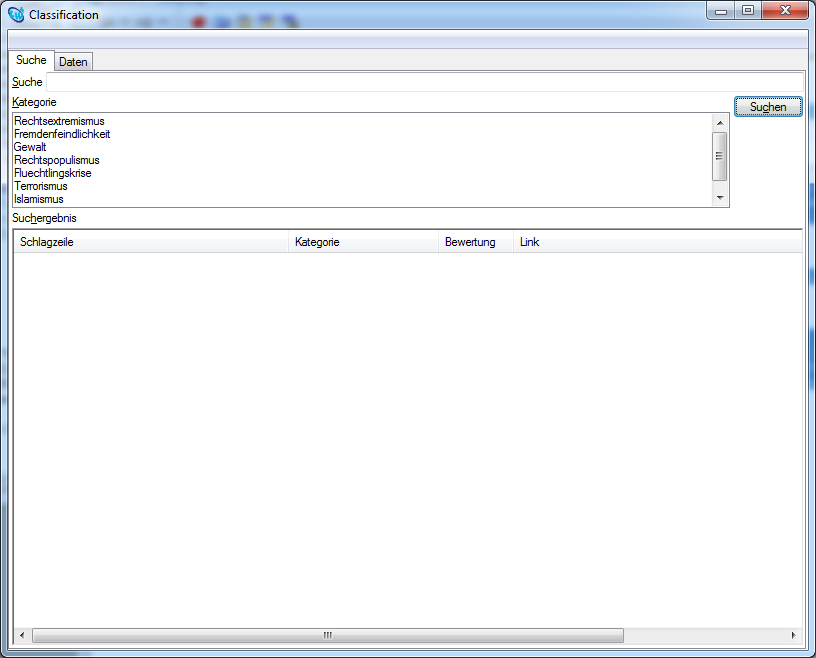
\includegraphics[width=\textwidth]{images/gui_main}}
	\end{minipage}
	\caption{Hauptfenster der Anwendung}
	\label{gui_main}
\end{figure}

%Nach Hauptfenster

\begin{figure}[h!]
\begin{minipage}{\linewidth}
	\centering
	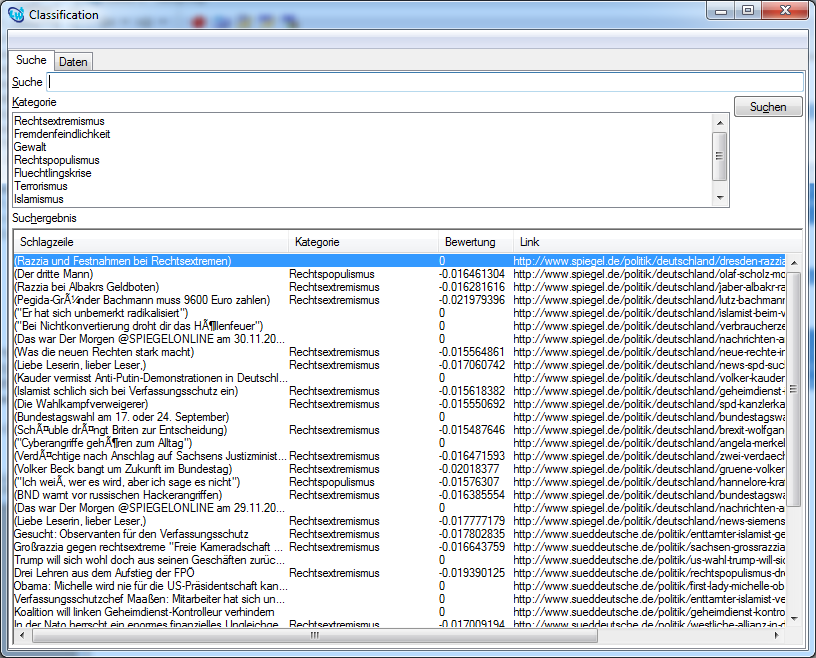
\includegraphics[width=\textwidth]{images/gui_main_result}
		\end{minipage}
	\caption{Ergebnis einer Suche ohne Filterung}
	\label{gui_result}
\end{figure}

Bei der Suche gibt es drei verschiedene M�glichkeiten.
Die einfachste Variante ist, dass weder nach Schlagworten noch nach Kategorien gefiltert wird.

Die Suche beschr�nkt sich dabei auf die aktuellen Artikel der Kategorien \textit{Politk} beziehungsweise \textit{Deutschlandpolitik}, der Online-Nachrichtenportale \textit{S�ddeutsche} und \textit{Spiegel}.
Dies ist in der Abbildung \ref{gui_result} dargestellt.


\begin{figure}[h!]
\begin{minipage}{\linewidth}
	\centering
	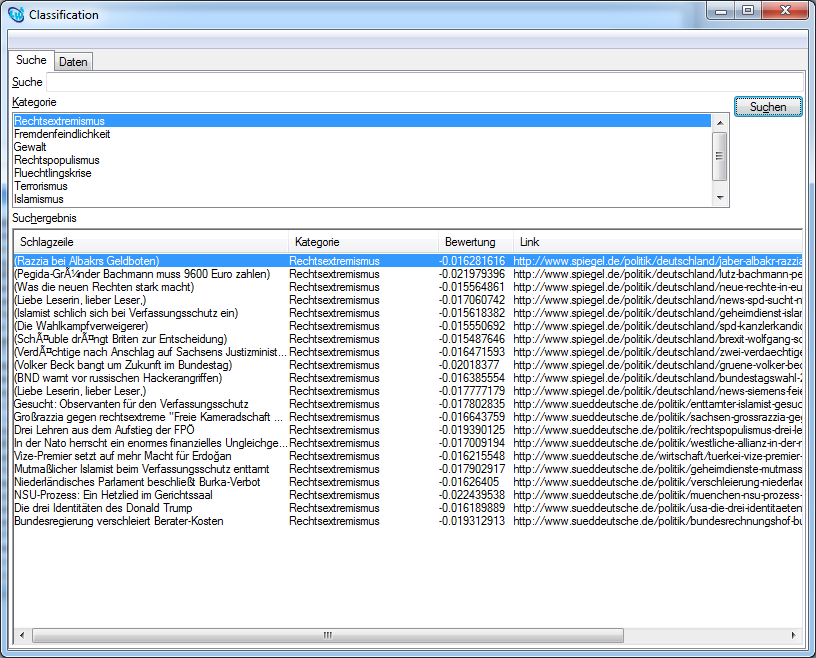
\includegraphics[width=\textwidth]{images/gui_main_result_filtered}
		\end{minipage}
	\caption{Ergebnis einer Suche, gefiltert nach der Kategorie "`Rechtsextremismus"'}
	\label{gui_result_filtered}
\end{figure}

Wurden eine oder mehrere Kategorien ausgew�hlt, so werden nur Artikel, die einer dieser Kategorien zugewiesen werden konnten, angezeigt.

Diese Filterung erm�glicht eine effiziente Suche nach Themen, die f�r den Anwender von Interesse sind, ohne Artikel durchzusehen, die keinen inhaltlichen Bezug zum Interessengebiet haben.

Im letzten Anwendungsfall gibt es die M�glichkeit, zus�tzlich nach Schlagworten zu filtern. Dabei wird der Artikeltext nach Vorkommnissen durchsucht. Da diese Suche allerdings keine intelligente Suche darstellt, muss diese auf grobe Schlagworte begrenzt sein und bietet nicht die M�glichkeit zusammenh�ngende S�tze oder W�rter gezielt zu suchen. 
Allerdings erm�glicht dies eine bessere Filterung nach beispielsweise Personen �ffentlichen Interesses, die in den durchsuchten Artikeln erscheinen k�nnten.

\newpage
\subsection{Daten}


Auf dem zweiten Reiter \textit{Daten} (siehe Abbildung \ref{gui_main_data}) k�nnen die vordefinierten Klassen in einer Baumstruktur eingesehen werden. Diese listet alle zugeh�rigen Dokumente 
sowie die mit diesen assozierten Artikel auf.

\newpage
Wird ein Element ausgew�hlt, werden die Symbol-Attribute angezeigt mit denen Details ersichtlich sind.\\

\begin{figure}[h!]
	\begin{minipage}{\linewidth}
		\centering
		\makebox[\linewidth]{
			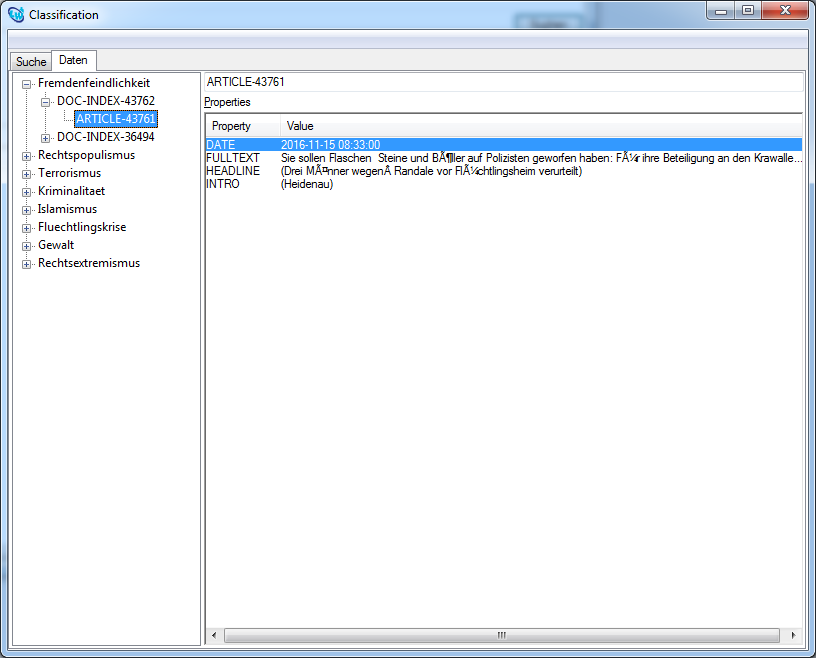
\includegraphics[width=\textwidth]{images/gui_main_data}}
		\caption{�berblick �ber die vordefinierten Klassen}
		\label{gui_main_data}
	\end{minipage}
\end{figure}

Diese Informationen erm�glichen es zu pr�fen, ob die vordefinierten Kategorien entsprechend der Planung durch die Konfigurationsdateien erstellt wurden und liefern einen Einblick in die dahinterliegenden Datenstrukturen.
\newpage
\section{Benutzung der entwickelten Software}

In diesem Kapitel wird erl�utert, wie die erstellte Software zu starten ist und welche Rahmenbedingungen daf�r erf�llt sein m�ssen.

\subsection{Voraussetzungen}

Um das erstellte Programm nutzen zu k�nnen muss die Entwicklungsumgebung \textit{LispWorks} mit Versionsnummer 6.+ installiert sein, sowie eine Internetverbindung vorhanden sein.
Mit �lteren \textit{LispWorks}-Versionen ist die Programmausf�hrung nicht m�glich und mit Versionen ab Nummer 7.0 ist die Anwendung nicht getestet und es ist nicht garantiert, dass alle Funktionen fehlerfrei arbeiten.
Um das Programm in vollen Umfang nutzen zu k�nnen bietet sich die sogenannte \textit{Professional}-Version and, da diese keine Speicher-Begrenzung hat. Dies tritt bei der kostenfreien \textit{Personal}-Edition auf und kann zu Programmabst�rzen f�hren, da \textit{LispWorks} automatisch beendet wird wenn eine gewisse Speichergrenze �berschritten wird, was bei einer gr��eren Menge an Trainingsdaten passiert.
In diesem Fall ist es n�tig mit einer kleineren Testmenge zu arbeiten, eine Anleitung daf�r ist in der im folgenden Kapitel beschriebenen Setup-Datei hinterlegt.

\subsection{Programmstart}

Um die Anwendung zu starten muss die im \textit{src}-Ordner befindliche Datei \textit{setup.lisp} mit \textit{LispWorks} ge�ffnet werden.
Wird der Inhalt dieser Datei evaluiert �ffnet sich die im Kapitel \ref{chap-gui} beschriebene graphische Benutzeroberfl�che.
Sollte dies nicht der Fall sein, so sind in der Datei Kommentare hinterlegt, die dabei helfen das Programm erfolgreich zu starten.

Der Programmstart kann einige Minuten in Anspruch nehmen, da der gesamte Klassifikationskorpus erstellt werden muss. Die daf�r verantwortliche Codestelle ist folgende:
\begin{figure}[h!]
\begin{lstlisting}
(data:build-classificator (current-pathname "../data/categories" "txt") 
						(current-pathname "../data/structure" "txt") 
					  (list (current-pathname "../data/new-data" "txt")))
\end{lstlisting}
\caption{Funktion die den Klassifikationskorpus erstellt}
\label{build-class}
\end{figure}

Um einen k�rzeren Programmstart zu erm�glichen kann die in Zeile 3 (Abbildung \ref{build-class}) angegebene Trainingsdatei "`../data/new-data"' durch "`../data/spiegel-data"' ersetzt werden. Dies kann die Startzeit halbieren, sorgt allerdings auch f�r eine ungenauere Klassifikation.

Wird dies getan, muss der in Kapitel \ref{sec:doc-class} erw�hnte Schwellwert zur Klassifikation angepasst werden, da dieser von der L�nge der Trainingsdaten abh�ngig ist.
Dies wird in der Setupdatei mithilfe der Konstante \textit{*classification-value*} getan. Dieser muss ein Wert zwischen -1 und 0 zugewiesen werden. In der Setup-Datei befinden sich mehrere m�gliche Einstellungen dieser Konstante, die f�r die beigef�gten Trainingsdaten relativ gut gew�hlt wurden.

%\chapter{LaTeX-Bausteine}\label{Stile}

Der Text wird in bis zu drei Ebenen gegliedert:

\begin{enumerate}
  \item Kapitel ( \verb \chapter{Kapitel} ), \index{Kapitel}
  \item Unterkapitel  ( \verb \section{Abschnitt} ) und
  \item Unterunterkapitel  ( \verb \subsection{Unterabschnitte} ).
\end{enumerate}

\section{Abschnitt}\index{Abschnitt}
Text der Gliederungsebene 2.


\subsection{Unterabschnitt} \index{Unterabschnitt}
Text der Gliederungsebene 3.
Text Text Text Text Text Text Text Text Text Text Text Text Text Text Text
Beispiel f�r Quelltext\index{Quelltext} \\[2 ex]
\noindent
\begin{minipage}{1.0\textwidth} \small
\begin{lstlisting}
	Prozess 1:
	
	Acquire();
		a := 1;
	Release();
	...
	Acquire();
	if(b == 0)
	{					
		c := 3;
		d := a;
	}				
	Release();
\end{lstlisting}
\end{minipage}

\vspace{2cm}
\noindent
\begin{minipage}{1.0\textwidth} \small
\begin{lstlisting}
	Prozess 2:
	
	Acquire();
		b := 1;
	Release();
	...
	Acquire();
	if(a == 0)
	{					
		c := 5;
		d := b;
	}				
	Release();
\end{lstlisting}
\end{minipage}
\vskip 1em

Gr��ere Code-Fragmente sollten im Anhang eingef�gt werden.

\section{Abbildungen und Tabellen}

Abbildung\index{Abbildung} und Tabellen\index{Tabelle} werden zentriert eingef�gt. Grunds�tzlich sollen sie
erst dann erscheinen, nach dem sie im Text angesprochen wurden (siehe Abb. \ref{a1}). Abbildungen und Tabellen (siehe Tabelle \ref{t1}) k�nnen
im (flie�enden) Text (\verb here ), am Seitenanfang (\verb top ), am Seitenende
(\verb bottom ) oder auch gesammelt auf einer nachfolgenden Seite (\verb page )
oder auch ganz am Ende der Ausarbeitung erscheinen. Letzteres sollte man nur
dann w�hlen, wenn die Bilder g�nstig zusammen zu betrachten sind und die
Ausarbeitung nicht zu lang ist ($< 20$ Seiten).

%\begin{figure} %[hbtp]
%	\centering
%		\includegraphics{images/p1ReadSeq.pdf}
%	\caption{Bezeichnung der Abbildung}
%	\label{a1}
%\end{figure}

\begin{table} %[hbtp]
	\centering
		\begin{tabular}{l | l l l l}
		\textbf{Prozesse} & \textbf{Zeit} $\rightarrow$ \\
		\hline
			$P_{1}$ & $W(x)1$ \\
			$P_{2}$ & & $W(x)2$ \\
			$P_{3}$ & & $R(x)2$ & & $R(x)1$\\
			$P_{4}$ & & & $R(x)2$ & $R(x)1$\\
		\end{tabular}
	\caption{Bezeichnung der Tabelle}
	\label{t1}
\end{table}


\section{Mathematische Formel}\index{Formel}
Mathematische Formeln bzw. Formulierungen k�nnen sowohl im
laufenden Text (z.B. $y=x^2$) oder abgesetzt und zentriert im Text
erscheinen. Gleichungen sollten f�r Referenzierungen nummeriert
werden (siehe Formel \ref{gl-1}).
\begin{equation}
\label{gl-1}
e_{i}=\sum _{i=1}^{n}w_{i}x_{i}
\end{equation}

Entscheidungsformel:

\begin{equation}
\psi(t)=\left\{\begin{array}{ccc}
1 &  \qquad 0 <= t < \frac{1}{2} \\
-1 &  \qquad \frac{1}{2} <= t <1 \\
0 & \qquad sonst
\end{array} \right.
\end{equation}


Matrix:\index{Matrix}
\begin{equation}
A = \left(
\begin{array}{llll}
a_{11} & a_{12} & \ldots & a_{1n} \\
a_{21} & a_{22} & \ldots & a_{2n} \\
\vdots & \vdots & \ddots & \vdots \\
a_{n1} & a_{n2} & \ldots & a_{nn} \\
\end{array}
\right)
\end{equation}

Vektor:\index{Vektor} 

\begin{equation}
\overline{a} = \left(
\begin{array}{c}
a_{1}\\
a_{2}\\
\vdots\\
a_{n}\\
\end{array}
\right)
\end{equation}

\section{S�tze, Lemmas und Definitionen}\index{Satz}\index{Lemma}\index{Definition}

S�tze, Lemmas, Definitionen, Beweise,\index{Beweis} Beispiele\index{Beispiel} k�nnen in speziell daf�r vorgesehenen Umgebungen erstellt werden.

\begin{definition}(Optimierungsproblem)

Ein \emph{Optimierungsproblem} $\mathcal{P}$ ist festgelegt durch ein Tupel
$(I_\mathcal{P}, sol_\mathcal{P}, m_\mathcal{P}, goal)$ wobei gilt

\begin{enumerate}
\item $I_\mathcal{P}$ ist die Menge der Instanzen,
\item $sol_\mathcal{P} : I_\mathcal{P} \longmapsto \mathbb{P}(S_\mathcal{P})$ ist eine Funktion, die jeder Instanz $x \in I_\mathcal{P}$ eine Menge zul�ssiger L�sungen zuweist,
\item $m_\mathcal{P} : I_\mathcal{P} \times S_\mathcal{P} \longmapsto \mathbb{N}$ ist eine Funktion, die jedem Paar $(x,y(x))$ mit $x \in I_\mathcal{P}$ und $y(x) \in sol_\mathcal{P}(x)$ eine
Zahl $m_\mathcal{P}(x,y(x)) \in \mathbb{N}$ zuordnet (= Ma� f�r die L�sung $y(x)$ der Instanz $x$), und
\item $goal \in \{min,max\}$.
\end{enumerate}

\end{definition}

\begin{example} MINIMUM TRAVELING SALESMAN (MIN-TSP)
\begin{itemize}
\item $I_{MIN-TSP} =_{def}$ s.o., ebenso $S_{MIN-TSP}$
\item $sol_{MIN-TSP}(m,D) =_{def} S_{MIN-TSP} \cap \mathbb{N}^m$ 
\item $m_{MIN-TSP}((m,D),(c_1, \ldots , c_m)) =_{def} \sum_{i=1}^{m-1} D(c_i, c_{i+1}) + D(c_m,c_1)$ 
\item $goal_{MIN-TSP} =_{def} min$
\end{itemize}
\begin{flushright}
$\qed$
\end{flushright}
\end{example}

\begin{theorem} Sei $\mathcal{P}$ ein \textbf{NP}-hartes Optimierungsproblem.
Wenn $\mathcal{P} \in$ \textbf{PO}, dann ist \textbf{P} = \textbf{NP}.
\end{theorem}

\begin{proof} Um zu zeigen, dass \textbf{P} = \textbf{NP} gilt, gen�gt es
wegen Satz A.30 zu zeigen, dass ein einziges \textbf{NP}-vollst�ndiges
Problem in \textbf{P} liegt. Sei also $\mathcal{P}'$ ein beliebiges \textbf{NP}-vollst�ndiges Problem.

Weil $\mathcal{P}$ nach Voraussetzung \textbf{NP}-hart ist, gilt insbesondere
$\mathcal{P}' \leq_T \mathcal{P}_C$. Sei $R$ der zugeh�rige
Polynomialzeit-Algorithmus dieser Turing-Reduktion.
Weiter ist $\mathcal{P} \in$ \textbf{PO} vorausgesetzt, etwa verm�ge eines
Polynomialzeit-Algorithmus $A$. Aus den beiden
Polynomialzeit-Algorithmen $R$ und $A$ erh�lt man nun
leicht einen effizienten Algorithmus f�r $\mathcal{P}'$: Ersetzt man
in $R$ das Orakel durch $A$, ergibt dies insgesamt eine polynomielle
Laufzeit. 
%\begin{flushright}
$\qed$
% \end{flushright}
\end{proof}

\begin{lemma} Aus \textbf{PO} $=$ \textbf{NPO} folgt \textbf{P} $=$ \textbf{NP}.
\end{lemma}

\begin{proof} Es gen�gt zu zeigen, dass unter der angegeben
Voraussetzung KNAPSACK $\in$ \textbf{P} ist.

Nach Voraussetung ist MAXIMUM KNAPSACK $\in$ \textbf{PO},
d.h. die Berechnung von $m^*(x)$ f�r jede Instanz $x$ ist
in Polynomialzeit m�glich. Um KNAPSACK bei Eingabe
$(x,k)$ zu entscheiden, m�ssen wir nur noch $m^*(x) \geq k$
pr�fen. Ist das der Fall, geben wir $1$, sonst $0$ aus. Dies
bleibt insgesamt ein Polynomialzeit-Algorithmus. 
\begin{flushright}
$\qed$
\end{flushright}
\end{proof}

\section{Fu�noten}

In einer Fu�note k�nnen erg�nzende Informationen\footnote{Informationen die f�r die Arbeit zweitrangig sind, jedoch f�r den Leser interessant sein k�nnten.} angegeben werden. Au�erdem kann eine Fu�note auch Links enthalten. Wird in der Arbeit eine Software (zum Beispiel Java-API\footnote{\url{http://java.sun.com/}}) eingesetzt, so kann die Quelle, die diese Software zur Verf�gung stellt in der Fu�note angegeben werden.

\section{Literaturverweise}\index{Literatur}
Alle benutzte Literatur wird im Literaturverzeichnis angegeben\footnote{Dazu wird ein sogennanter bib-File, literatur.bib verwendet.}. Alle angegebene Literatur sollte mindestens einmal im Text referenziert werden\cite{Coulouris:02}.
%\chapter{Beispiel-Kapitel}

In diesem Kapitel wird beschrieben, warum es unterschiedliche Konsistenzmodelle\index{Konsistenzmodelle} gibt. Au�erdem werden die Unterschiede zwischen strengen Konsistenzmodellen\index{Linearisierbarkeit} (Linearisierbarkeit, sequentielle Konsistenz)\index{sequentiell!Konsistenz} und schwachen Konsistenzmodellen\index{Konsistenz!schwach} (schwache Konsistenz, Freigabekonsistenz)\index{Freigabekonsistenz} erl�utert. Es wird gekl�rt, was Strenge und Kosten (billig, teuer) in Zusammenhang mit Konsistenzmodellen bedeuten.

\section{Warum existieren unterschiedliche Konsistenzmodelle?}

Laut \cite{Malte:97} sind mit der\index{Replikation} Replikation von Daten immer zwei gegens�tzliche Ziele verbunden: die Erh�hung der\index{Verf�gbarkeit} Verf�gbarkeit und die Sicherung der\index{Konsistenz} Konsistenz der Daten. Die Form der Konsistenzsicherung bestimmt dabei, inwiefern das eine Kriterium erf�llt und das andere dementsprechend nicht erf�llt ist (Trade-off zwischen Verf�gbarkeit und der Konsistenz der Daten). Stark konsistente Daten sind stabil, das hei�t, falls mehrere Kopien der Daten existieren, d�rfen keine Abweichungen auftreten. Die Verf�gbarkeit der Daten ist hier jedoch stark eingeschr�nkt. Je schw�cher die Konsistenz wird, desto mehr Abweichungen k�nnen zwischen verschiedenen Kopien einer Datei auftreten, wobei die Konsistenz nur an bestimmten Synchronisationspunkten gew�hrleistet wird. Daf�r steigt aber die Verf�gbarkeit der Daten, weil sie sich leichter replizieren lassen.

Nach \cite{Mosberger:93} kann die Performanzsteigerung der schw�cheren Konsistenzmodelle wegen der Optimierung\index{Optimierung} (Pufferung, Code-Scheduling, Pipelines) 10-40 Prozent betragen. Wenn man bedenkt, dass mit der Nutzung der vorhandenen Synchronisierungsmechanismen schw�chere Konsistenzmodelle den Anforderungen der strengen Konsistenz gen�gen, stellt sich der h�here programmiertechnischer Aufwand bei der Implementierung der schw�cheren Konsistenzmodelle als ihr einziges Manko dar.

In \cite{Cheriton:85} ist beschrieben, wie man sich Formen von DSM vorstellen k�nnte, f�r die ein beachtliches Ma� an\index{Inkonsistenz} Inkonsistenz akzeptabel w�re. Beispielsweise k�nnte DSM verwendet werden, um die Auslastung von Computern in einem Netzwerk zu speichern, so dass Clients f�r die Ausf�hrung ihrer Applikationen die am wenigsten ausgelasteten Computer ausw�hlen k�nnen. Weil die Informationen dieser Art innerhalb k�rzester Zeit ungenau werden k�nnen (und durch die Verwendung der veralteten Daten keine gro�en Nachteile entstehen k�nnen), w�re es vergebliche M�he, sie st�ndig f�r alle Computer im System konsistent zu halten \cite{Coulouris:02}. Die meisten Applikationen stellen jedoch strengere Konsistenzanforderungen.

\section{Klassifizierung eines Konsistenzmodells}

Die zentrale Frage, die f�r die Klassifizierung\index{streng}\index{schwach} (streng oder schwach) eines Konsistenzmodells von Bedeutung ist \cite{Coulouris:02}: wenn ein Lesezugriff auf eine Speicherposition erfolgt, welche Werte von Schreibzugriffen auf diese Position sollen dann dem Lesevorgang bereitgestellt werden? Die Antwort f�r das schw�chste Konsistenzmodell lautet: von jedem Schreibvorgang, der vor dem Lesen erfolgt ist, oder in der "`nahen"' Zukunft, innerhalb des definierten Betrachtungsraums, erfolgten wird. Also irgendein Wert, der vor oder nach dem Lesen geschrieben wurde.

F�r das strengste Konsistenzmodell, Linearisierbarkeit (atomic consistency), stehen alle geschriebenen Werte allen Prozessoren sofort zur Verf�gung: eine Lese-Operation gibt den aktuellsten Wert zur�ck, der geschrieben wurde, bevor das Lesen stattfand. Diese Definition ist aber in zweierlei Hinsicht problematisch. Erstens treten weder Schreib- noch Lese-Operationen zu genau einem Zeitpunkt auf, deshalb ist die Bedeutung von "`aktuellsten"' nicht immer klar. Zweitens ist es nicht immer m�glich, genau festzustellen, ob ein Ereignis vor einem anderen stattgefunden hat, da es Begrenzungen daf�r gibt, wie genau Uhren in einem verteilten System synchronisiert werden k�nnen.

Nachfolgend werden einige Konsistenzmodelle absteigend nach ihrer Strenge vorgestellt. Zuvor m�ssen wir allerdings kl�ren, wie die Lese- und Schreibe-Operationen in dieser Ausarbeitung dargestellt werden.

Sei $x$ eine Speicherposition, dann k�nnen Instanzen dieser Operationen wie folgt ausgedr�ckt werden:
\begin{itemize}
	\item $R(x)a$ - eine Lese-Operation\index{Operation!Lese}, die den Wert $a$ von der Position $x$ liest.
	\item $W(x)b$ - eine Schreib-Operation\index{Operation!Schreib}, die den Wert $b$ an der Position $x$ speichert.
\end{itemize}

\section{Linearisierbarkeit\index{Linearisierbarkeit} (atomic consistency)}

Die Linearisierbarkeit im Zusammenhang mit DSM kann wie folgt definiert werden:
\begin{itemize}
	\item Die verzahnte Operationsabfolge findet so statt: wenn $R(x)a$ in der Folge vorkommt, dann ist die letzte Schreib-Operation, die vor ihr in der verzahnten Abfolge auftritt, $W(x)a$, oder es tritt keine Schreib-Operation vor ihr auf und $a$ ist der Anfangswert von $x$. Das bedeutet, dass eine Variable nur durch eine Schreib-Operation ge�ndert werden kann.
	\item Die Reihenfolge der Operationen in der Verzahnung ist konsistent zu den \underline{Echtzeiten}\index{Echtzeiten}, zu denen die Operationen bei der tats�chlichen Ausf�hrung aufgetreten sind.
\end{itemize}

Die Bedeutung dieser Definition kann an folgendem Beispiel (Tabelle \ref{tab:1}) nachvollzogen werden. Es sei angenommen, dass alle Werte mit $0$ vorinitialisiert sind.

\begin{table}
	\centering
		\begin{tabular}{l | l l l l}
			\textbf{Prozesse} & \textbf{Zeit} $\rightarrow$ & \\
			\hline
			$P_{1}$ & $W(x)1$ & & $W(y)2$ \\
			$P_{2}$ & & $R(x)1$ & & $R(y)2$ \\
		\end{tabular}
	\caption{Linearisierbarkeit ist erf�llt}
	\label{tab:1}
\end{table}

Hier sind beide Bedingungen erf�llt, da die Lese-Operationen den zuletzt geschriebenen Wert zur�ckliefern. Interessanter ist es, zu sehen, wann die Linearisierbarkeit verletzt ist.

\begin{table}
	\centering
		\begin{tabular}{l | l l l l}
		\textbf{Prozesse} & \textbf{Zeit} $\rightarrow$ \\
		\hline
		$P_{1}$ & $W(x)1$ & $W(x)2$ \\
		$P_{2}$ & & & \color{red} $R(x)0$ & \color{black} $R(x)2$ \\
		\end{tabular}
	\caption{Linearisierbarkeit ist verletzt, sequentielle Konsistenz ist erf�llt.}
	\label{tab:2}
\end{table}

In diesem Beispiel (Tabelle \ref{tab:2}) ist die Echtzeit-Anforderung verletzt, da der Prozess $P_{2}$ immer noch den alten Wert liest, obwohl er von Prozess $P_{1}$ bereits ge�ndert wurde. Diese Ausf�hrung w�re aber sequentiell konsistent (siehe kommender Abschnitt), da es eine Verzahnung der Operationen gibt, die diese Werte liefern k�nnte ($R(x)0$, $W(x)1$, $W(x)2$, $R(y)2$). W�rde man beide Lese-Operationen des 2. Prozesses vertauschen, wie in der Tabelle \ref{tab:3} dargestellt, so w�re keine sinnvolle Verzahnung mehr m�glich.

\begin{table}
	\centering
		\begin{tabular}{l | l l l l}
		\textbf{Prozesse} & \textbf{Zeit} $\rightarrow$ \\
		\hline
		$P_{1}$ & $W(x)1$ & $W(x)2$ \\
		$P_{2}$ & & & \color{red} $R(x)2$ &  \color{red} $R(x)0$ \\
			
		\end{tabular}
	\caption{Linearisierbarkeit und sequentielle Konsistenz sind verletzt.}
	\label{tab:3}
\end{table}

In diesem Beispiel sind beide Bedingungen verletzt. Selbst wenn die Echtzeit, zu der die Operationen stattgefunden haben, ignoriert wird, gibt es keine Verzahnung einzelner Operationen, die der Definition entsprechen w�rde.
\chapter{Zusammenfassung}

%In diesem Kapitel soll die Arbeit noch einmal kurz zusammengefasst werden. Insbesondere sollen die wesentlichen Ergebnisse Ihrer Arbeit herausgehoben werden. Erfahrungen, die z.B. Benutzer mit der Mensch-Maschine-Schnittstelle gemacht haben oder Ergebnisse von Leistungsmessungen sollen an dieser Stelle pr�sentiert werden. Sie k�nnen in diesem Kapitel auch die Ergebnisse oder das Arbeitsumfeld Ihrer Arbeit kritisch bewerten. W�nschenswerte Erweiterungen sollen als Hinweise auf weiterf�hrende Arbeiten erw�hnt werden.

Das in dieser Arbeit erstellte Programm erm�glicht es, erfolgreich Artikel in passende Kategorien einzuordnen und somit eine gute Filterung von Nachrichtenartikel zu erzielen.
Problematisch ist diese Kategorisierung allerdings bez�glich der Auswahl der Trainingsdaten. So ist zum einen eine sehr gro�e Menge an Artikeln notwendig um eine genaue Klassifikation zu erm�glichen, doch ist dies auch mit einem gro�en Aufwand verbunden. Die in dieser Arbeit erstellten Trainingsdaten sind nicht Umfangreich genug um eine wirklich zufriedenstellende Kategorisierung zu erm�glichen, zeigen aber auch das Potenzial des Algorithmus.\\

Insgesamt l�sst sich diese Arbeit als Erfolg werten. Die zugrunde liegenden Algorithmen sind voll funktionsf�hig und die Aufteilung der Programmpakete erm�glicht eine einfache Wartung und Erweiterung.
Der intensive Kontakt mit verschiedenen Verfahren zur Textklassifikation und anderen Data-Mining Algorithmen hat bei mir die Absicht geweckt sich noch weiter mit diesem Themengebiet zu besch�ftigen und die genannten Verbesserungen des Programms in Zukunft zu realisieren.

%ausf�hrlicher?

\newpage
\chapter{Ausblick}

Die erstellte Anwendung hat viel Potenzial f�r Verbesserungen, so wird beispielsweise der erstellte Klassifikationskorpus nicht gespeichert und muss bei jedem Programmstart neu erstellt werden, was mit einer mehrmin�tigen Wartezeit verbunden ist.
Desweiteren ist die Abdeckung von nur zwei Nachrichtenportalen nicht optimal, kann aber durch die hier entworfene Bezeichnungssprache relativ einfach erweitert werden.\\
Eine weitere m�gliche Verbesserung w�re es, die schon durchsuchten Artikel abzuspeichern und somit eine M�glichkeit zur Archivierung und langfristigen Verbesserung der Trainingsdaten zu erm�glichen. Die Suche k�nnte ebenso ausgeweitet werden, da sie sich zurzeit nur auf die auf der ersten Seite einer angegebenen Nachrichtenseite bezieht und �ltere Artikel nicht durchsucht. Dies greift mit der erw�hnten Archivierung zusammen, da so schon klassifizierte Artikel nicht erneut gepr�ft werden m�ssten.\\

Denkbar w�re auch eine Erweiterung die es erm�glicht auch andere Quellen zu klassifizieren, beispielsweise eingescannte Dokumente oder Magazine die mithilfe einer Texterkennungssoftware vorverarbeitet werden. So w�rde das Programm nicht nur von Online-Medien abh�ngig sein und w�rde Optionen bieten ein umfassendes Archiv aufzubauen.
Hierf�r k�nnte eine erweiterte Hierarchie sinnvoll sein, die es erlaubt auch Ober- beziehungsweise Unterkategorien zu definieren, mit denen die Kategorisierung und Suche verfeinert werden k�nnte.\\

Da der Klassifikationsalgorithmus mit einem simplen \textit{Bag-of-Words}-Modell arbeitet, der lediglich einzelne W�rter verwendet, k�nnte auch �ber eine m�gliche Verwendung von \textit{N-Grammen} nachgedacht werden. Dies bedeutet statt jeweils ein Wort zu z�hlen, \textit{N} W�rter zu z�hlen und dann zu klassifizieren. Es k�nnte ausgewertet werden ob dies eine Verbesserung erbringt oder nicht. 
Insgesamt k�nnen basierend auf dieser Arbeit viele solcher Optionen ber�cksichtigt werden. Die verwendeten Metriken k�nnen mit der im Kapitel \ref{chap-ext-bayes} beschriebenen Optionen ausgetauscht werden und dann mithilfe von weiteren Testdaten die f�r Nachrichtenartikel beste Methode zu evaluieren.


% ...
%--------------------------------------------------------------------------
\backmatter                        		% Anhang
%-------------------------------------------------------------------------
\bibliographystyle{geralpha}			% Literaturverzeichnis
\bibliography{literatur}     			% BibTeX-File literatur.bib
%--------------------------------------------------------------------------
\printindex 							% Index (optional)
%--------------------------------------------------------------------------
\begin{appendix}						% Anh�nge sind i.d.R. optional
   %\chapter{Glossar}

\abbreviation{DisASTer}		{DisASTer (Distributed Algorithms Simulation Terrain), A platform for the Implementation of Distributed Algorithms}
\abbreviation{DSM}			{Distributed Shared Memory}
\abbreviation{AC}			{Linearisierbarkeit (atomic consistency)}
\abbreviation{SC}			{Sequentielle Konsistenz (sequential consistency)}
\abbreviation{WC}			{Schwache Konsistenz (weak consistency)}
\abbreviation{RC}			{Freigabekonsistenz (release consistency)}
			% Glossar   
   \chapter{Erkl�rung der Kandidatin / des Kandidaten}

\begin{description}[$\Box$~]
\item[$\Box$] Die Arbeit habe ich selbstst�ndig verfasst und keine anderen als die angegebenen Quellen- und Hilfsmittel verwendet.\\

\item[$\Box$] Die Arbeit wurde als Gruppenarbeit angefertigt. Meine eigene Leistung ist\\
...\\

Diesen Teil habe ich selbstst�ndig verfasst und keine anderen als die angegebenen Quellen und Hilfsmittel verwendet. \\

Namen der Mitverfasser: ...

\end{description}

\vspace{2cm}

\begin{minipage}[t]{3cm}
\rule{3cm}{0.5pt}
Datum
\end{minipage}
\hfill
\begin{minipage}[t]{9cm}
\rule{9cm}{0.5pt}
Unterschrift der Kandidatin / des Kandidaten
\end{minipage}	% Selbstst�ndigkeitserkl�rung
\end{appendix}

\end{document}
